\newpage
\appendix
\section{Appendix}

% === A.1 Efficiency ===
\subsection{Implementation Details and Computational Efficiency}
\label{subsec:implementation}

\paragraph{Training details.} Our training protocol employs cosine learning rate decay with a 1,000-step warmup, gradient accumulation across 4 steps, a batch size of 32 per preference pair, and precision bf16 training. Training proceeds for a minimum of 5 epochs, with validation performed every 50 steps, and model checkpoints saved at the same interval.

{
\paragraph{Computational Efficiency Analysis.} 
We analyze the runtime costs for both inference (deployment) and training (development) to demonstrate the practicality of the framework.
\begin{itemize}
    \item \textbf{Inference Latency:} We benchmarked inference speeds on a single \textbf{NVIDIA RTX A6000 GPU} using the 4FE5 backbone (Length=67). For a batch size of 8, RiboPO (based on gRNAde) required 5.29 seconds ($\approx 0.66$ s/seq). This is comparable to the diffusion baseline RiboDiffusion \citep{huang2024ribodiffusion}, which required 2.68s with 50 denoising steps ($\approx 0.34$ s/seq) and 4.73s with 100 denoising steps ($\approx 0.59$ s/seq). While diffusion speed varies with step count ($T$), RiboPO's autoregressive generation provides deterministic runtime scaling with length ($L$), offering competitive throughput without the need to tune denoising hyperparameters.
    
    \item \textbf{Preference Pair Construction (Offline):} RiboPO utilizes an offline RL strategy, decoupling physical feedback from gradient updates. The construction of the preference dataset ($\sim 14,000$ pairs) is the primary computational bottleneck due to the cost of 3D structure prediction. This process required approximately 3 days using a 32-core Intel Xeon Gold 6530 CPU, utilizing RhoFold+ \citep{shen2024accurate} for structure prediction.
    
    \item \textbf{Training Time and Convergence:} Once preference data is pre-computed, the DPO fine-tuning is efficient. A single round of training (10 epochs) requires approximately 16 hours on a single NVIDIA A100 GPU. We observed that the model converges rapidly, reaching stability in validation preference accuracy at approximately 8,000 gradient steps. This indicates high sample efficiency compared to online RL methods that often require millions of samples. For each sample, RhoFold+ predicts the 3D structure at around 0.14s (without MSA), and thus acting as an efficient proxy tool. 

    \item \textbf{Sample Efficiency (The "Hit Rate" Payoff):} While RiboPO incurs an offline training cost, it significantly reduces the deployment cost. As shown in our Pass@k analysis, RiboPO achieves an 11\% higher hit rate than the baseline. Consequently, a user needs to sample and fold fewer sequences to find a valid design, significantly reducing the "Total Time to Success" in experimental or in silico workflows.
\end{itemize}

\paragraph{Asymptotic Time Complexity.}
Let $L$ denote backbone length, $K$ the number of backbone conformations, and $T$ the number of denoising steps in a diffusion sampler. Both gRNAde and RiboPO use a $k$-nearest-neighbour geometric graph with $k = O(1)$ and a fixed number of GNN layers, so $|E| = O(L)$ and a single encoder--decoder forward pass scales as $O(KL)$. Generating $M$ sequences with RiboPO or gRNAde therefore costs $O(MKL)$, and DPO fine-tuning over $N_{\text{pair}}$ preference pairs has total cost $O(N_{\text{pair}} K L)$, up to a constant factor for the number of epochs. In contrast, RiboDiffusion \citep{huang2024ribodiffusion} applies its backbone network for $T$ denoising steps, so sampling a single sequence scales as $O(TL)$, introducing an explicit multiplicative factor $T$ compared to the single-pass autoregressive cost. Finally, offline preference construction is dominated by external structure and energy predictions: if $C_{\text{3D}}(L)$ and $C_{\text{2D/thermo}}(L)$ denote the costs of 3D and thermodynamic engines for length $L$, constructing a dataset with $N_G$ backbones and $N_{\text{cand}}$ candidates per backbone has cost $O\!\big(N_G N_{\text{cand}} (C_{\text{3D}}(L) + C_{\text{2D/thermo}}(L))\big)$, which is a one-time offline expense reused across all DPO training runs.



% === A.2 SSTT Definitions (SIMPLIFIED) ===
\subsection{SSTT: Comprehensive Fine-Grained RNA Design}
\label{subsec:sstt_detail}

\vspace{0.5ex}
\noindent\textbf{Notation.} For a candidate sequence $y=(y_1,\dots,y_L)$ and the native sequence $y^{\mathrm{nat}}$, let $S_0$ denote the target secondary structure. Partition-function outputs are base-pair probabilities $p_{ij}$ and unpaired probabilities $q_i$. Predicted 3D coordinates are $\mathbf{X}(y)$; native/target coordinates are $\mathbf{X}^{\mathrm{ref}}$.

\subsection*{Sequence axis (S)}
\begin{itemize}[leftmargin=1.2em,itemsep=2pt,topsep=2pt]
\item \textbf{Recovery} \citep{dauparas2022proteinmpnn}: Recovery measures the average percentage of native nucleotides correctly recovered in the sampled sequences. It is computed as
$$\mathrm{Rec}(y) \;=\; \frac{1}{L} \sum_{i=1}^{L} \mathbb{1}\{y_i = y_i^{\mathrm{nat}}\}.$$

\item \textbf{Perplexity} ($\downarrow$, lower-is-better) \citep{bengioaneural}: Perplexity measures how well a model predicts the sequences. Given a model (reference or policy) with token probabilities $p_\theta$, perplexity is defined as the average exponential of the negative log-likelihood of the sampled sequences.
$$\mathrm{PPL}(y) \;=\; \exp\!\Big(-\frac{1}{L} \sum_{i=1}^{L} \log p_\theta(y_i \mid y_{<i}, \mathcal{G})\Big).$$

\item \textbf{Diversity (3-mer)} ($\uparrow$): Given $n$ candidates for the backbone $\mathcal{G}$, let $v_s \in \mathbb{R}^{64}$ be the normalized 3-mer frequency of candidate $s$. Define
$$\mathrm{Div}_{3\mathrm{mer}}(\mathcal{G}) \;=\; 1 \;-\; \frac{2}{n(n-1)} \sum_{1 \le s < t \le n} \rho\!\big(v_s, v_t\big),$$
where $\rho(\cdot,\cdot)$ is the Pearson correlation. It's the quantification of sequence variety based on substring frequency distributions \citep{shannon1948mathematical, Bokulich2024diversitykmer}.
\end{itemize}

\subsection*{Secondary axis (S) — forward-folding self-consistency}
\begin{itemize}[leftmargin=1.2em,itemsep=2pt,topsep=2pt]
\item \textbf{2D (EternaFold) scMCC (Matthews Correlation Coefficient) \citep{matthews1975comparison}} ($\uparrow$): This metric measures the ability of designs to recover base pairing patterns. We use EternaFold \citep{waymentsteele2022eternafold} to perform forward folding on the sampled sequences and then calculate the Matthews correlation coefficient (MCC) by comparing the predicted base-pair adjacency matrix with the ground truth.
\end{itemize}

\subsection*{Thermostability axis (T) — ensemble specificity}
\begin{itemize}[leftmargin=1.2em,itemsep=2pt,topsep=2pt]
\item \textbf{MFE} (kcal/mol, $\downarrow$): The minimum free energy (MFE) of the most stable predicted secondary structure. \emph{Note:} MFE is a single-structure quantity and does not capture ensemble specificity; we therefore also report Ensemble defect per nucleotide (ED/nt).

\item \textbf{Ensemble defect (ED) \citep{zadeh2011nucleic} and ED/nt} ($\downarrow$): The ensemble defect (ED) measures the discrepancy between the predicted base-pair probabilities and the true structural states.
\[
\mathrm{ED}(y;S_0)=\sum_{i\in U_0}(1-q_i)+\sum_{i\in P_0}\big(1-p_{i\,j^*(i)}\big),\qquad \mathrm{ED/nt}=\mathrm{ED}/L.
\]
\end{itemize}

\subsection*{Tertiary axis (T)}
\begin{itemize}[leftmargin=1.2em,itemsep=2pt,topsep=2pt]
\item \textbf{TM-score} \citep{zhang2004tmscore} ($\uparrow$): Evaluates structural alignment quality using US-align \citep{zhang2022usalign}.
$$
\mathrm{TM}(y) \;=\; \frac{1}{L_{\mathrm{ref}}} \sum_{i=1}^{L_{\mathrm{ali}}} \frac{1}{1 + \left(\frac{d_i}{d_0(L_{\mathrm{ref}})}\right)^2},
\quad
d_0(L) \;=\; 1.24\sqrt[3]{L-15}-1.8.
$$

\item \textbf{pLDDT} ($\uparrow$): The mean predicted LDDT confidence \citep{jumper2021alphafold2}.
\item \textbf{RMSD} ($\downarrow$): Root-Mean-Square Deviation of the atomic coordinates.
\item \textbf{INF (ALL)} \citep{parisien2009newmetricsinf} ($\uparrow$): Interaction-network fidelity assessing base-pairing accuracy.
\item \textbf{Clash score} ($\downarrow$): Number of all-atom steric clashes per 1000 atoms \citep{word1999clashscore}.
\end{itemize}

% === A.3 Full Results Extended (Trimmed to match A.2) ===
% 

% === A.3 Full Results Extended ===
\subsection{{Full RiboPO SSTT Results and Baselines (Extended)}}
\label{sec:full_results_appendix}

{
Table \ref{tab:sstt_extended} presents the extended set of SSTT metrics not reported in the main text. This includes sequence diversity, global structure quality (GDT), thresholded success rates, confidence scores (pLDDT), interaction fidelity (INF), stereochemical feasibility (Clash Score), and ensemble specificity (ED/nt).

\begin{table}[htbp]
\centering
\caption{Extended SSTT Benchmark Results. This table complements Main Table 1 by reporting additional metrics for Diversity, Tertiary Quality (GDT, pLDDT, INF), Stereochemistry (Clash Score), and Ensemble Specificity (ED/nt). RiboPO (Round 2) demonstrates the best balance of diversity ($0.87$) and structural confidence (pLDDT $0.65$), while maintaining low steric clashes and competitive ensemble defects.}
\label{tab:sstt_extended}
\resizebox{\textwidth}{!}{
\begin{tabular}{lccccccccc}
\toprule
\textbf{Model} & \textbf{Div} (3-mer) $\uparrow$ & \textbf{GDT} $\uparrow$ & \textbf{\%GDT $\ge$ 0.5} $\uparrow$ & \textbf{\%TM $\ge$ 0.45} $\uparrow$ & \textbf{pLDDT} $\uparrow$ & \textbf{\%pLDDT $\ge$ 0.7} $\uparrow$ & \textbf{INF} (ALL) $\uparrow$ & \textbf{Clash} $\downarrow$ & \textbf{ED/nt} $\downarrow$ \\
\midrule
RiFold                      & 0.89 & 0.121 & 0.012 & 0.024 & 0.502 & 0.012 & 0.39 & 678.3 & 0.0034 \\
RDesign                     & 0.84 & 0.124 & 0.024 & 0.012 & 0.453 & 0.024 & 0.38 & 740.6 & 0.0036 \\
% R3Design\textsuperscript{*} & 0.41 & 0.470 & 0.554 & 0.578 & 0.678 & 0.542 & 0.58 & 569.5 & 0.0023 \\
% RiboDiffusion\textsuperscript{*} & 0.22 & 0.633 & 0.868 & 0.838 & 0.768 & 0.824 & 0.65 & 504.7 & 0.0025 \\
% RhoDesign\textsuperscript{*} & 0.62 & 0.272 & 0.263 & 0.250 & 0.559 & 0.289 & 0.49 & 685.0 & 0.0069 \\
RIDiffusion                 & 0.85 & 0.272 & 0.157 & 0.168 & 0.609 & 0.282 & 0.52 & 644.0 & 0.0626 \\
gRNAde (Base)               & 0.82 & 0.285 & 0.286 & 0.301 & 0.621 & 0.381 & 0.48 & 637.5 & 0.0028 \\
\midrule
RiboPO Round 1              & \textbf{0.90} & 0.291 & 0.273 & 0.302 & \textbf{0.655} & \textbf{0.450} & \textbf{0.50} & \textbf{595.5} & \textbf{0.0021} \\
RiboPO Round 2              & 0.87 & \textbf{0.314} & \textbf{0.301} & \textbf{0.325} & 0.652 & 0.449 & 0.49 & 617.9 & 0.0043 \\
RiboPO Round 4              & 0.89 & 0.280 & 0.239 & 0.287 & 0.646 & 0.424 & 0.49 & 613.6 & 0.0043 \\
\bottomrule
\end{tabular}
}
% \par\small\emph{* Baselines with test-set overlap; values may be inflated due to leakage.}
\end{table}
}



% === A.4 De-duplication ===
\subsection{{Evaluation on De-duplicated Benchmark}}
\label{subsec:dedup}

{
To ensure a rigorous evaluation free from data leakage, we re-evaluated all models on a strictly de-duplicated subset of the test set. We removed from DAS testing dataset any RNA targets that appeared in the training sets of baseline models and then evaluate those baseline models on the rest. The results are reported in Table \ref{tab:clean_benchmark}.

\begin{table}[htbp]
\centering
\caption{Performance comparison on the strict De-duplicated Test Set. RiboPO achieves the best balance of structural fidelity (RMSD) and thermodynamic stability (MFE) without relying on data leakage.}
\label{tab:clean_benchmark}
\resizebox{\textwidth}{!}{
\begin{tabular}{lcccccc}
\toprule
\textbf{Model} & \textbf{Seq Rec} & \textbf{scMCC} (2D) ($\uparrow$) & \textbf{RMSD} (\AA) ($\downarrow$) & \textbf{\%RMSD $\leq$ 8\AA} ($\uparrow$) & \textbf{TM-score} ($\uparrow$) & \textbf{MFE} (kcal/mol) ($\downarrow$) \\
\midrule
RDesign       & 0.42 & 0.21 & 16.48 & 0.23 & 0.13 & -22.06 \\
R3Design      & 0.51 & 0.59 & 14.52 & 0.47 & 0.27 & -26.57 \\
RhoDesign     & 0.47 & 0.21 & 14.82 & 0.18 & 0.14 & -13.53 \\
RiboDiffusion & 0.52 & 0.49 & 13.52 & 0.25    & 0.22 & -20.28 \\
gRNAde (Base) & \textbf{0.53} & 0.61 & 11.43 & 0.29 & 0.29 & -32.84 \\
\midrule
\textbf{RiboPO (Round 2)} & 0.50 & \textbf{0.70} & \textbf{10.23} & \textbf{0.51} & \textbf{0.31} & \textbf{-36.86} \\
\bottomrule
\end{tabular}
}
\end{table}
}

% === A.5 Pareto Analysis ===
\subsection{{Pareto Frontier Analysis of Multi-Objective Trade-offs}}
\label{subsec:pareto}

{
To analyze the trade-off between structural fidelity, thermodynamic stability, and sequence recovery, we performed a Pareto analysis across training rounds and varying $\beta$ hyperparameters. Figure \ref{fig:pareto} illustrates the movement of the model in the multi-objective space.

\begin{figure}[htbp]
    \centering
    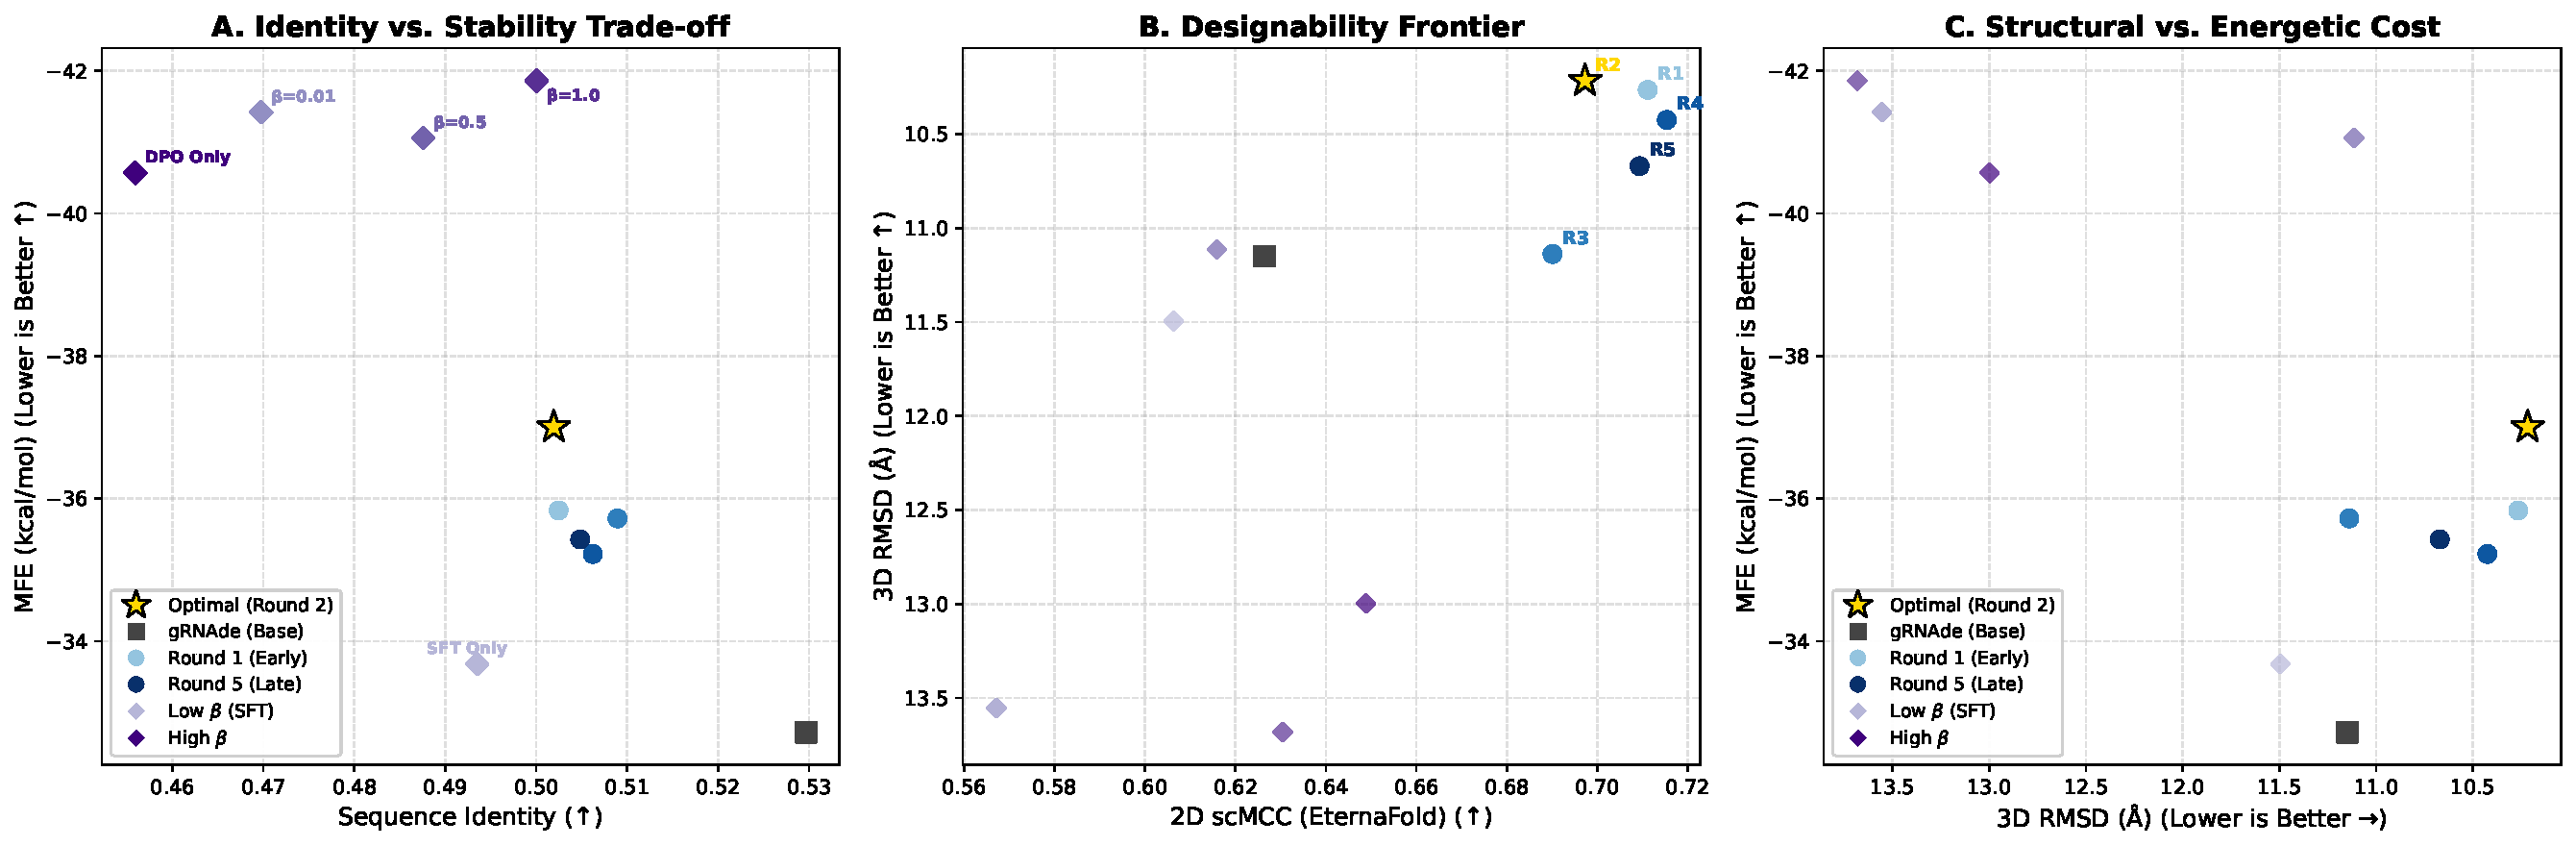
\includegraphics[width=\textwidth]{figs/pareto_analysis.pdf}
    \caption{\textbf{Pareto Frontier Analysis.} (A) Sequence Identity vs. MFE trade-off. (B) Designability Frontier (scMCC vs. RMSD). (C) Structural vs. Energetic Cost. RiboPO (Round 2, Star) represents the optimal operating point.}
    \label{fig:pareto}
\end{figure}

\paragraph{Analysis.} 
\begin{itemize}
    \item \textbf{Designability Frontier (Figure \ref{fig:pareto}B):} The base model (gRNAde, square) sits in a sub-optimal region. RiboPO Round 2 (Star) pushes the frontier significantly towards the top-left (Higher scMCC, Lower RMSD), indicating an expanded "designable basin." Later rounds (R3-R5) continue to improve MFE but show diminishing returns on structural consistency.
    \item \textbf{Identity vs. Stability (Figure \ref{fig:pareto}A):} We observe a slight drop in sequence recovery ($\sim 3\%$) correlated with a massive improvement in MFE ($12.3\%$). This confirms that the model is exploring non-native, thermodynamically favorable regions of the sequence space rather than failing to learn.
\end{itemize}
}

% === A.6 Cross-Tool Robustness ===
\subsection{{Cross-Tool Robustness Evaluation}}
\label{subsec:robustness}

{
To address concerns that RiboPO might be overfitting to the specific energy function used during training (ViennaRNA), we evaluated the generated sequences using two external thermodynamic engines: NUPACK \citep{Fornace2022NUPACK} and RNAstructure \citep{RNAstructure_tool2013}. 

As shown in Table \ref{tab:crosstool}, the stability improvements generalize well. RiboPO sequences show a $10.15\%$ improvement in MFE under NUPACK and a $12.32\%$ improvement under RNAstructure compared to the baseline. This confirms that the method learns generalized thermodynamic stability principles rather than tool-specific artifacts.

\begin{table}[htbp]
\centering
\caption{Cross-Tool Robustness. MFE improvements generalize to NUPACK and RNAstructure engines, validating biophysical robustness.}
\label{tab:crosstool}
\begin{tabular}{lccc}
\toprule
\textbf{Method} & \textbf{\textit{NUPACK} MFE} & \textbf{\textit{RNAstructure} MFE} & \textbf{Improv. (\small{\textit{NUPACK} / \textit{RNAstructure}} \%)} \\
\midrule
gRNAde (Base)   & -28.90 & -30.53 & - \\
RiboPO (Round 2) & -31.84 & -34.29 & \textbf{+10.2\% / +12.3\%} \\
\bottomrule
\end{tabular}
\end{table}



\paragraph{3D Structural Generalization.}
We assessed the structural fidelity of sequences generated by the gRNAde base model and RiboPO (Round 2) using AlphaFold3 \citep{abramson2024accurate} and DRFold2 \citep{li2025drfold2}. These tools employ folding algorithms distinct from the RhoFold+ engine used in our reward loop, serving as different proxies. 

As shown in Table~\ref{tab:3d_robustness}, RiboPO consistently outperforms the baseline across all independent evaluators. Notably, evaluation with AlphaFold3—currently considered the gold standard in biomolecular structure prediction—reveals that RiboPO designs achieve lower RMSD (2.81 \AA{} vs. 3.00 \AA{}) and higher TM-scores (0.43 vs. 0.41) compared to the baseline. This improvement on unseen predictors indicates that the RLPF framework steers the policy toward universally valid structural basins rather than merely exploiting artifacts of the training surrogate.

It's also worth-noting that AlphaFold3 and DRFold2 output better self-consistency scores on the de-duplicated dataset, but performed complementary results on individual samples \citep{Martin2024review}, indicating that the RNA 3D structure prediction hasn't arrived the "AlphaFold Moment" \citep{li2025drfold2}. We'd like to call for the development of better RNA structure prediction models by the structure prediction community, and to claim that with better 3D structure prediction tools, our RiboPO/RLPF can have less biased feedback and output more meaningful RNA designs.

\begin{table}[h]
    \centering
    \caption{\textbf{3D Cross-Tool Robustness.} Evaluation of generated sequences using independent structure predictors (AlphaFold3 and DRFold2) not seen during training. Across all the mentioned tools, RiboPO (Multi-Round 2) demonstrates consistent structural improvements over the baseline, validating that the geometric gains are model-agnostic.}
    \label{tab:3d_robustness}
    \vspace{0.2cm}
    \resizebox{0.8\textwidth}{!}{
    \begin{tabular}{l|ccc|cc}
        \toprule
        & \multicolumn{3}{c|}{\textbf{AlphaFold 3}} & \multicolumn{2}{c}{\textbf{DRFold 2}} \\
        \textbf{Model} & \textbf{RMSD} ($\downarrow$) & \textbf{TM-Score} ($\uparrow$) & \textbf{pLDDT} ($\uparrow$) & \textbf{RMSD} ($\downarrow$) & \textbf{TM-Score} ($\uparrow$) \\
        \midrule
        gRNAde (Base) & 3.00 & 0.41 & 61.02 & 2.96 & 0.37 \\
        \textbf{RiboPO (Round 2)} & \textbf{2.81} & \textbf{0.43} & \textbf{62.05} & \textbf{2.79} & \textbf{0.39} \\
        \bottomrule
    \end{tabular}
    }
\end{table}




% === A.7 Native Structure Eval ===
\subsection{{Native Structure Evaluation Benchmark}}
\label{subsec:native}

{
To contextualize the performance of all models, we report the evaluation metrics on the native ground-truth sequences in Table \ref{tab:native}. These values represent the "upper bound" (or target) for current predictors (RhoFold/EternaFold).

\begin{table}[htbp]
\centering
\caption{{Evaluation of Native Sequences (Ground Truth). Note that non-zero RMSD arises from the use of structure predictors (RhoFold) on native sequences. These values serve as the upper bound for current prediction tools.}}
\label{tab:native}
\resizebox{\textwidth}{!}{
\begin{tabular}{lcccccccccc}
\toprule
\textbf{Sequence} & \textbf{Seq Rec} & \textbf{scMCC} & \textbf{RMSD} (\AA) & \textbf{\%RMSD $\leq$ 8\AA} & \textbf{TM-score} & \textbf{\%TM $\ge$ 0.45} & \textbf{pLDDT} & \textbf{\%pLDDT $\ge$ 0.70} & \textbf{MFE} & \textbf{ED/nt} \\
\midrule
Native & 1.00 & 0.86 & 5.78 & 0.82 & 0.56 & 0.65 & 0.74 & 0.72 & -42.83 & 0.002 \\
\bottomrule
\end{tabular}
}
\end{table}
}


\subsection{{Statistical Significance and Variance Analysis}}
\label{subsec:variance}

{
To ensure that the reported improvements are robust and not artifacts of random initialization, we evaluated the optimal RiboPO model (Round 2) and the baseline gRNAde across 4 independent random seeds ($0, 6, 40, 42$). Table \ref{tab:variance} reports the mean and standard deviation ($\mu \pm \sigma$) for key performance metrics.

RiboPO demonstrates consistent superiority in thermodynamic stability (MFE: $-36.98$ vs. $-32.71$) and structural consistency (scMCC: $0.69$ vs. $0.62$) with low variance. Crucially, we observe statistically significant gains in tertiary structure confidence (pLDDT: $0.65$ vs. $0.63$), validating that the preference optimization improves the density of high-quality designs.

\begin{table}[htbp]
\centering
\caption{Variance Analysis across 4 random seeds ($N=4$). Values represent Mean $\pm$ Standard Deviation. RiboPO achieves statistically significant improvements across both structural and thermodynamic axes.}
\label{tab:variance}
\resizebox{\textwidth}{!}{
\begin{tabular}{lcccccc}
\toprule
\textbf{Model} & \textbf{Seq Rec} & \textbf{scMCC} & \textbf{RMSD} (\AA) $\downarrow$ & \textbf{TM-score} $\uparrow$ & \textbf{pLDDT} $\uparrow$ & \textbf{MFE} (kcal/mol) $\downarrow$ \\
\midrule
gRNAde (Base) & $0.531 \pm 0.004$ & $0.625 \pm 0.015$ & $11.17 \pm 0.22$ & $0.297 \pm 0.003$ & $0.626 \pm 0.004$ & $-32.71 \pm 0.12$ \\
\textbf{RiboPO (R2)} & $0.502 \pm 0.001$ & $\mathbf{0.694 \pm 0.007}$ & $\mathbf{10.31 \pm 0.25}$ & $\mathbf{0.307 \pm 0.009}$ & $\mathbf{0.649 \pm 0.004}$ & $\mathbf{-36.98 \pm 0.13}$ \\
\bottomrule
\end{tabular}
}
\end{table}
}


% === Placeholders ===
% \subsection{{Theoretical Analysis}}
% \label{subsec:theory}
% {
% [Placeholder: Theoretical analysis of the RiboPO optimization landscape and complexity will be added here.]
% }






























% \subsection{Theoretical Analysis}
% \label{app:theory}

% In this subsection we provide a theoretical perspective on RiboPO/RLPF.
% We (i) formalize our preference construction in terms of an underlying
% multi-objective physical reward and an ``ideal'' Boltzmann distribution over
% stable sequences, (ii) connect the DPO training objective with a \emph{fixed
% reference policy} to a KL-regularized variational problem in which the base
% model acts as a prior, (iii) relate the multi-round training scheme to
% iterative refinement of this objective and movement into designable basins,
% and (iv) discuss multi-objective trade-offs, Goodhart-type effects, and the
% role of biased surrogate predictors and the SFT anchor.

% \subsubsection{Latent multi-objective reward and Boltzmann view}

% For each backbone $G$, we associate a sequence $s$ with a vector of normalized
% physical features
% \begin{equation}
%     \phi(s, G) \in \mathbb{R}^d,
% \end{equation}
% including tertiary-structure quality (e.g.\ RMSD, pLDDT), secondary-structure
% self-consistency (e.g.\ scMCC), and thermodynamic proxies (e.g.\ MFE,
% ensemble defect, target-structure probability, entropy, melting temperature),
% as defined in the main text. We assume there exists a latent
% \emph{multi-objective} reward function
% \begin{equation}
%     r(s, G) \;=\; w^\top \phi(s, G),
%     \qquad w \succeq 0,
%     \label{eq:latent-reward}
% \end{equation}
% that encodes the relative importance of structural fidelity and
% thermodynamic stability in RNA inverse folding.

% A particularly interpretable special case is obtained by defining a composite
% physical energy function
% \begin{equation}
%     E(s, G)
%     =
%     \lambda_{\text{thermo}} \, E_{\text{thermo}}(s)
%     +
%     \lambda_{\text{geom}} \, E_{\text{geom}}(s, G),
% \end{equation}
% where $E_{\text{thermo}}$ aggregates thermodynamic terms (e.g.\ MFE and
% ensemble measures) and $E_{\text{geom}}$ penalizes structural deviations
% (e.g.\ RMSD). Setting $r(s,G) = -E(s,G)$ recovers a standard Boltzmann form.

% Let $p^*(s \mid G)$ denote an ``ideal'' physical distribution over sequences
% for backbone $G$, defined by a Boltzmann distribution
% \begin{equation}
%     p^*(s \mid G)
%     \;\propto\;
%     \exp\bigl\{-\beta E(s, G)\bigr\}
%     \;=\;
%     \exp\bigl\{\beta r(s, G)\bigr\},
%     \label{eq:boltzmann-physical}
% \end{equation}
% for some inverse temperature $\beta > 0$.
% In our setting, we also have a strong backbone-conditioned autoregressive
% base model $\pi_{\text{ref}}(s \mid G)$ (gRNAde), which we can view as a
% data-driven prior over plausible sequences for $G$. Combining the prior
% with the energy-based likelihood yields a target distribution
% \begin{equation}
%     q^*(s \mid G)
%     \;\propto\;
%     \pi_{\text{ref}}(s \mid G)\,\exp\bigl\{\beta r(s, G)\bigr\}.
%     \label{eq:target-posterior}
% \end{equation}
% Thus, an ideal optimizer would transform the base model $\pi_{\text{ref}}$
% into a posterior-like policy $q^*$ that favors sequences with high
% structural and thermodynamic reward while remaining close to the data
% manifold learned by $\pi_{\text{ref}}$.

% Our preference construction is designed to be consistent with such a reward.
% We first apply a \emph{feasibility gate} that enforces that a candidate
% winner $s_w$ lies in a physically plausible region:
% \begin{equation}
%     \operatorname{pLDDT}(g(s_w)) > \kappa, \qquad
%     \operatorname{RMSD}(G, g(s_w)) < \gamma, \qquad
%     \operatorname{MFE}(s_w) < \delta,
%     \label{eq:gate}
% \end{equation}
% where $g(\cdot)$ is the structure predictor and
% $\kappa, \gamma, \delta$ are thresholds.
% Second, for each feasible pair $(s_w, s_l)$ we enforce margin
% conditions on structural and thermodynamic deltas:
% \begin{align}
%     \bigl|\operatorname{pLDDT}(s_w) - \operatorname{pLDDT}(s_l)\bigr|
%     &> \gamma_r \sigma_{\text{pLDDT}},
%     \label{eq:margin-plddt}
%     \\
%     \bigl|\operatorname{RMSD}(s_w) - \operatorname{RMSD}(s_l)\bigr|
%     &> \gamma_r \sigma_{\text{RMSD}},
%     \label{eq:margin-rmsd}
%     \\
%     \operatorname{MFE}(s_w) &< \operatorname{MFE}(s_l),
%     \label{eq:margin-mfe}
% \end{align}
% where $\sigma_m$ is the empirical scale of metric $m(\cdot)$ and
% $\gamma_r$ controls how strict the preference is in round $r$.
% These conditions exclude candidates unlikely to fold correctly and filter out
% near-equivalent pairs where metric differences are on the same order as
% predictor noise, improving the signal-to-noise ratio of the implicit reward.
% Normalization by $\sigma_m$ renders metrics on different scales commensurate
% and stabilizes the DPO likelihood-ratio updates.

% Because the components of $\phi$ are normalized and we only retain pairs
% for which $s_w$ is strictly better on at least one structural feature and
% strictly better in energy, there exists a non-negative weight vector
% $w \succeq 0$ such that
% \begin{equation}
%     r(s_w, G) - r(s_l, G) \;\geq\; \Delta_r \;>\; 0
%     \label{eq:reward-gap}
% \end{equation}
% for all retained pairs $(G, s_w, s_l)$. In the special case $r=-E$, this is
% equivalent to requiring $E(s_w,G) < E(s_l,G)$ by a margin, i.e.\ the winner
% is stochastically more stable.

% We can therefore model our preferences using a standard
% Bradley--Terry--Luce (BTL) logistic model. Let
% $s_w \succ s_l$ denote the event that $s_w$ is preferred over $s_l$.
% We posit that, conditional on $G$,
% \begin{equation}
%     \mathbb{P}(s_w \succ s_l \mid G)
%     \;=\;
%     \sigma\!\left(
%         \beta \bigl(
%             r(s_w, G) - r(s_l, G)
%         \bigr)
%     \right),
%     \label{eq:btl}
% \end{equation}
% where $\sigma$ denotes the logistic sigmoid and
% $\beta > 0$ is an inverse-temperature parameter.
% In the idealized noiseless case, the gating and margins ensure that
% $r(s_w, G) - r(s_l, G) > 0$ for all pairs, so the empirical preferences are
% consistent with a single latent reward $r$ (or equivalently a single
% energy function $E$ via $r=-E$).

% \subsubsection{DPO with a fixed reference as KL-regularized variational inference}

% Let $\pi_\theta(s \mid G)$ denote the policy parameterized by RiboPO,
% and $\pi_{\text{ref}}(s \mid G)$ the fixed reference policy (the base gRNAde
% model). For each preference triple $(G, s_w, s_l)$, the DPO loss used in
% RiboPO is
% \begin{equation}
%     L_{\text{DPO}}(\theta)
%     =
%     -\mathbb{E}_{(G, s_w, s_l)}
%     \left[
%         \log \sigma\!\left(
%             \beta
%             \Big(
%                 \log \pi_\theta(s_w \mid G) - \log \pi_\theta(s_l \mid G)
%                 -\log \pi_{\text{ref}}(s_w \mid G) + \log \pi_{\text{ref}}(s_l \mid G)
%             \Big)
%         \right)
%     \right].
%     \label{eq:dpo-loss}
% \end{equation}
% We additionally apply a supervised fine-tuning (SFT) anchor on the winners:
% \begin{equation}
%     L_{\text{SFT}}(\theta)
%     =
%     - \mathbb{E}_{(G,s_w)} \bigl[ \log \pi_\theta(s_w \mid G) \bigr],
%     \label{eq:sft-loss}
% \end{equation}
% and train RiboPO with the combined objective
% \begin{equation}
%     L(\theta) = L_{\text{DPO}}(\theta) + \lambda_{\text{SFT}} L_{\text{SFT}}(\theta),
%     \label{eq:combined-loss}
% \end{equation}
% where $\lambda_{\text{SFT}} \geq 0$ controls the strength of the anchor.

% Although the optimization problem we implement is written entirely in terms of
% the preference cross-entropy \eqref{eq:dpo-loss} and the SFT term
% \eqref{eq:sft-loss}, the \emph{population optimum} of the DPO part admits a
% useful variational characterization. Under the BTL model \eqref{eq:btl} with
% reward $r(s,G)$, the unique policy $\pi^*$ that exactly matches the induced
% preferences can be written in closed form as
% \begin{equation}
%     \pi^*(s \mid G)
%     \;\propto\;
%     \pi_{\text{ref}}(s \mid G)
%     \exp\bigl\{\beta r(s, G)\bigr\}.
%     \label{eq:boltzmann-posterior}
% \end{equation}
% Comparing \eqref{eq:boltzmann-posterior} with \eqref{eq:target-posterior}
% shows that $\pi^*$ coincides with the target posterior-like distribution $q^*$.
% Equivalently, $\pi^*$ is the unique minimizer of the KL divergence
% \begin{equation}
%     \pi^* \;=\; \arg\min_{\pi} \;
%     \mathbb{E}_{G}
%     \Bigl[
%         \mathrm{KL}\bigl(
%             \pi(\cdot \mid G)
%             \,\Vert\,
%             q^*(\cdot \mid G)
%         \bigr)
%     \Bigr],
%     \label{eq:kl-qstar}
% \end{equation}
% and the unique maximizer of the KL-regularized reward objective
% \begin{equation}
%     J(\pi)
%     =
%     \mathbb{E}_{G}
%     \left[
%         \mathbb{E}_{s \sim \pi(\cdot \mid G)} \bigl[r(s, G)\bigr]
%         -
%         \frac{1}{\beta}
%         \mathrm{KL}
%         \bigl(
%             \pi(\cdot \mid G)
%             \,\Vert\,
%             \pi_{\text{ref}}(\cdot \mid G)
%         \bigr)
%     \right].
%     \label{eq:kl-reg}
% \end{equation}
% Thus, while our training loss is expressed in terms of pairwise preference
% logistic losses, the corresponding population optimum can be interpreted as
% the solution to a KL-regularized physical reward maximization problem, or
% equivalently as variational inference that projects the base model
% $\pi_{\text{ref}}$ onto the physically informed target $q^*$.

% The fact that $\pi_{\text{ref}}$ is kept \emph{fixed} is crucial for this
% interpretation: the KL term in \eqref{eq:kl-reg} is always taken with respect
% to the same prior $\pi_{\text{ref}}$, so the objective $J(\pi)$ does not change
% over rounds. If the reference policy were instead updated to the current
% $\pi_\theta$ at each step, the center of the KL penalty would move, effectively
% weakening the prior over time and making it easier for the policy to drift
% toward reward-hacking regimes that exploit imperfections in the surrogate
% metrics. In contrast, a fixed $\pi_{\text{ref}}$ maintains a consistent
% trade-off between improving the physical reward and staying close to the
% data-driven prior over biologically plausible sequences.

% For intuition, consider the derivative of $L_{\text{DPO}}$ with respect to
% the log-probabilities of the winner and loser. Let
% \begin{equation}
%     z
%     =
%     \beta\left(
%         \log\frac{\pi_\theta(s_w \mid G)}{\pi_\theta(s_l \mid G)}
%         -
%         \log\frac{\pi_{\text{ref}}(s_w \mid G)}{\pi_{\text{ref}}(s_l \mid G)}
%     \right).
% \end{equation}
% Then
% \begin{equation}
%     \frac{\partial L_{\text{DPO}}}{\partial \log \pi_\theta(s_w \mid G)}
%     =
%     \beta \bigl(\sigma(z) - 1\bigr),
%     \qquad
%     \frac{\partial L_{\text{DPO}}}{\partial \log \pi_\theta(s_l \mid G)}
%     =
%     \beta \bigl(1 - \sigma(z)\bigr).
%     \label{eq:dpo-grads}
% \end{equation}
% When $\pi_\theta$ under-prefers the winner relative to the reference
% ($z$ small), $\sigma(z) \ll 1$ and the gradient increases
% $\log \pi_\theta(s_w \mid G)$ while decreasing $\log \pi_\theta(s_l \mid G)$.
% When $\pi_\theta$ already strongly prefers $s_w$ over $s_l$, $\sigma(z)
% \approx 1$ and the gradient vanishes. This yields a well-behaved optimization
% landscape in which only ``hard'' or ambiguous preferences drive learning.
% The SFT term \eqref{eq:sft-loss} then sharpens the mode of the learned
% policy around high-reward winners, mitigating reward hacking and mode collapse.

% \subsubsection{Multi-round training and designable basins}

% We now link this perspective to multi-round RLPF and the notion of
% designable basins. For a given backbone $G$, define the designable set of
% sequences
% \begin{equation}
%     \mathcal{S}_{\text{des}}(G)
%     =
%     \left\{
%         s :
%         \operatorname{RMSD}(G, g(s)) \le \tau_{\text{struct}},
%         \;
%         \operatorname{scMCC}(s, G) \ge \tau_{\text{struct}},
%         \;
%         \operatorname{MFE}(s) \le \tau_{\text{thermo}}
%     \right\},
%     \label{eq:designable-set}
% \end{equation}
% for suitable structural and thermodynamic thresholds
% $\tau_{\text{struct}}, \tau_{\text{thermo}}$.
% The \emph{designability} of $G$ under a policy $\pi$ is then
% \begin{equation}
%     D_\pi(G)
%     =
%     \sum_{s \in \mathcal{S}_{\text{des}}(G)} \pi(s \mid G),
%     \label{eq:designability}
% \end{equation}
% i.e., the total probability mass that $\pi$ assigns to sequences that fold
% accurately and occupy deep thermodynamic basins.

% By construction, the feasibility gate \eqref{eq:gate} ensures that winners
% $s_w$ lie in $\mathcal{S}_{\text{des}}(G)$ for appropriately chosen
% thresholds, while losers may lie inside or outside this set.
% The gradient updates in \eqref{eq:dpo-grads} therefore \emph{redistribute}
% probability mass from low-reward or infeasible sequences into
% $\mathcal{S}_{\text{des}}(G)$, increasing $D_\pi(G)$ over training.
% This formalizes the claim that RiboPO moves the policy toward more
% designable basins in sequence space.

% The multi-round training scheme further refines this process. Each round
% $r$ proceeds in two steps:
% \begin{enumerate}
%     \item Use the current policy $\pi_{\theta_{r-1}}$ to generate a pool of
%     candidate sequences for each backbone $G$.
%     \item Construct preference pairs from this pool using the same gating and
%     margin criteria, and update $\pi_{\theta_r}$ by minimizing
%     \eqref{eq:combined-loss} with \emph{the same} reference policy
%     $\pi_{\text{ref}}$.
% \end{enumerate}
% From the KL-regularized perspective \eqref{eq:kl-reg}, each round can be
% viewed as performing an approximate mirror-descent step on $J(\pi)$ from
% the previous policy, but always with the KL term centered at the fixed
% prior $\pi_{\text{ref}}$. The candidate-generation step enriches the support
% over which preferences are constructed: early rounds primarily explore
% regions favored by $\pi_{\text{ref}}$, whereas later rounds can propose
% sequences in newly discovered high-reward basins. The fixed reference
% ensures that, despite this exploration, all rounds optimize the \emph{same}
% trade-off between physical reward and fidelity to the base model.

% Empirically, this picture is consistent with the observation that intermediate
% rounds often lie near the Pareto front between recovery, structural, and
% thermodynamic metrics: early rounds move the policy from a purely
% data-driven prior toward physically favorable basins; later rounds refine
% within those basins but may over-specialize to small and noisy differences
% in surrogate metrics, leading to diminishing returns or regressions on some
% objectives.

% \subsubsection{Multi-objective trade-offs, Goodhart effects, and the SFT anchor}

% The latent reward $r(s,G)$ in \eqref{eq:latent-reward} is explicitly
% multi-objective: it combines structural fidelity (RMSD, scMCC, pLDDT) with
% thermodynamic terms (MFE and ensemble metrics). Optimizing such a scalarized
% reward inevitably induces trade-offs: improving one component (e.g.\ MFE)
% may worsen others (e.g.\ exact sequence recovery). This is reflected in the
% empirical Pareto-front analyses, where different choices of $\beta$ and
% round index yield different operating points.

% From a theoretical standpoint, over-optimizing a single proxy (e.g.\ MFE as
% a surrogate for true stability and biological plausibility) can lead to
% Goodhart-type failure modes: the optimizer exploits idiosyncrasies of the
% proxy and drifts toward unphysical, low-complexity structures that score
% well under the surrogate but are biologically implausible. Our framework
% mitigates this in three ways:

% \paragraph{Multi-objective reward.}
% First, preferences are only retained when the winner is at least as good on
% the structural metrics and strictly better in energy. This reduces the risk
% of collapsing onto thermodynamically trivial but structurally incorrect
% solutions.

% \paragraph{KL regularization against the base model.}
% Second, the KL-regularized objective \eqref{eq:kl-reg} shows that, in the
% idealized limit, DPO with a fixed reference seeks policies that improve
% $r(s,G)$ while remaining close to the base model $\pi_{\text{ref}}$. This
% discourages pathological modes that deviate drastically from the
% distribution of sequences seen in training, even if they exploit
% idiosyncrasies of the surrogate metrics.

% \paragraph{SFT as a distributional anchor.}
% Third, the SFT term \eqref{eq:sft-loss} acts as an explicit
% \emph{distributional anchor}. While the DPO component pulls the policy toward
% low-energy, structurally consistent sequences, the SFT component biases
% $\pi_\theta$ toward sequences similar to the winners produced by the base
% model. At a high level, the combined objective seeks a policy that (i)
% increases expected physical reward relative to $\pi_{\text{ref}}$ and (ii)
% stays on or near the manifold of sequences that are likely under a
% high-quality inverse folder. This theoretical balance explains the
% empirical trade-offs observed in our experiments: RiboPO is allowed to
% sacrifice a modest amount of exact sequence recovery to access regions of
% sequence space with improved structure and stability, but the KL and SFT
% anchors limit the extent to which the policy can exploit surrogate-specific
% artifacts.

% \subsubsection{Surrogate predictors, bias, and extensibility}

% Finally, we address the fact that RiboPO relies on imperfect and potentially
% biased surrogate predictors of RNA structure and energetics, and argue that
% the framework remains principled and extensible as stronger models become
% available.

% Let $r^*(s, G)$ denote an unknown ``true'' physical reward, e.g.\ derived
% from exact folding and thermodynamics or experimental measurements. We do
% not observe $r^*$ directly. Instead, we construct a surrogate reward
% $r_\Phi(s, G)$ based on a feature vector
% \begin{equation}
%     \Phi(s, G)
%     =
%     \bigl(
%         \phi^{\text{3D}}(s, G),
%         \phi^{\text{2D}}(s, G),
%         \phi^{\text{thermo}}(s, G),
%         \dots
%     \bigr),
% \end{equation}
% which aggregates outputs from multiple biophysical tools (e.g.\ RhoFold+,
% EternaFold, ViennaRNA).
% Our working reward can be written as
% \begin{equation}
%     r_\Phi(s, G) = w^\top \Phi(s, G),
%     \label{eq:surrogate-reward}
% \end{equation}
% for some non-negative weight vector $w$. Each component of $\Phi$ is a
% biased proxy for an underlying physical quantity, so we can decompose
% \begin{equation}
%     r_\Phi(s, G)
%     =
%     r^*(s, G) + \eta(s, G),
%     \label{eq:reward-bias}
% \end{equation}
% where $\eta$ captures the combined bias and noise of the surrogate predictors
% and the chosen weights.

% Our preference labels are generated by comparing $r_\Phi$:
% we declare $s_w$ preferred to $s_l$ if $r_\Phi(s_w,G) > r_\Phi(s_l,G)$ and
% the gating conditions hold. Let $s_w \succ^* s_l$ denote the ``true''
% preference according to $r^*$. We assume that, for pairs surviving the gate,
% the surrogate and true preferences are aligned with probability at least
% $1-\rho$:
% \begin{equation}
%     \mathbb{P}\Bigl(
%         \operatorname{sign}\bigl(r_\Phi(s_w, G) - r_\Phi(s_l, G)\bigr)
%         =
%         \operatorname{sign}\bigl(r^*(s_w, G) - r^*(s_l, G)\bigr)
%     \Bigr)
%     \;\geq\; 1 - \rho,
%     \qquad \rho < \tfrac{1}{2}.
%     \label{eq:alignment}
% \end{equation}
% Intuitively, even though individual predictors are imperfect, they rank
% higher-quality sequences above clearly worse ones more often than chance.
% Under this mild assumption, the expected gradient of the DPO objective is
% still correlated with the gradient of the true reward $r^*$: in aggregate,
% preference updates move the policy toward better $r^*$, albeit with some
% variance due to mis-specified or noisy labels.

% Crucially, the use of a \emph{vector} of surrogate features
% $\Phi(s,G)$ rather than a single tool reduces the risk of overfitting to any
% one predictor's bias. Only sequences that look consistently better across
% multiple, differently biased views (3D, 2D, thermodynamics) tend to survive
% the gating and margin filters and be chosen as winners. This multi-tool
% formulation is modular: as stronger predictors of RNA structure and
% energetics become available, they can be incorporated into $\Phi$ (or used
% to replace existing components) without changing the RLPF/RiboPO learning
% algorithm.

% In the idealized limit where
% $\sup_{s,G} \lvert r_\Phi(s,G) - r^*(s,G) \rvert \to 0$ as tools improve,
% the mis-ranking probability $\rho$ in \eqref{eq:alignment} tends to zero and
% the induced preferences converge to the true physical preferences. In this
% limit, DPO trained on preferences from $r_\Phi$ converges (in function space)
% to the same KL-regularized optimal policy one would obtain by training
% directly on $r^*$. Thus, the proposed RLPF/RiboPO framework can be viewed as
% a modular pipeline whose performance is guaranteed to systematically improve
% as biophysical surrogates become more accurate, while already yielding
% meaningful improvements under today's imperfect RNA structure and
% thermodynamics models.





\subsection{Theoretical Analysis}
\label{app:theory}

In this subsection we provide a theoretical perspective on RiboPO/RLPF.
We (i) formalize our preference construction in terms of an underlying
multi-objective physical reward and an ``ideal'' Boltzmann distribution over
stable sequences, (ii) connect the DPO training objective with a \emph{fixed
reference policy} to a KL-regularized variational problem in which the base
model acts as a prior, (iii) relate the multi-round training scheme to
iterative refinement of this objective and movement into designable basins,
and (iv) discuss multi-objective trade-offs, Goodhart-type effects, and the
role of biased surrogate predictors and the SFT anchor.

\subsubsection{Latent multi-objective reward and Boltzmann view}

For each backbone $G$, we associate a sequence $s$ with a vector of normalized
physical features
\begin{equation}
    \phi(s, G) \in \mathbb{R}^d,
\end{equation}
including tertiary-structure quality (e.g.\ RMSD, pLDDT), secondary-structure
self-consistency (e.g.\ scMCC), and thermodynamic proxies (e.g.\ MFE,
ensemble defect, target-structure probability, entropy, melting temperature),
as defined in the main text. We normalize and, when necessary, sign-flip
individual metrics so that larger values of each component of
$\phi(s,G)$ correspond to better structural fidelity or stability. We then
assume there exists a latent \emph{multi-objective} reward function
\begin{equation}
    r(s, G) \;=\; w^\top \phi(s, G),
    \qquad w \succeq 0,
    \label{eq:latent-reward}
\end{equation}
that encodes the relative importance of structural fidelity and
thermodynamic stability in RNA inverse folding.

A particularly interpretable special case is obtained by defining a composite
physical energy function
\begin{equation}
    E(s, G)
    =
    \lambda_{\text{thermo}} \, E_{\text{thermo}}(s)
    +
    \lambda_{\text{geom}} \, E_{\text{geom}}(s, G),
\end{equation}
where $E_{\text{thermo}}$ aggregates thermodynamic terms (e.g.\ MFE and
ensemble measures) and $E_{\text{geom}}$ penalizes structural deviations
(e.g.\ RMSD). Setting $r(s,G) = -E(s,G)$ recovers a standard Boltzmann form.

Let $p^*(s \mid G)$ denote an ``ideal'' physical distribution over sequences
for backbone $G$, defined by a Boltzmann distribution
\begin{equation}
    p^*(s \mid G)
    \;\propto\;
    \exp\bigl\{-\beta E(s, G)\bigr\}
    \;=\;
    \exp\bigl\{\beta r(s, G)\bigr\},
    \label{eq:boltzmann-physical}
\end{equation}
for some inverse temperature $\beta > 0$.
In our setting, we also have a strong backbone-conditioned autoregressive
base model $\pi_{\text{ref}}(s \mid G)$ (gRNAde), which we can view as a
data-driven prior over plausible sequences for $G$. Combining the prior
with the energy-based likelihood yields a target distribution
\begin{equation}
    q^*(s \mid G)
    \;\propto\;
    \pi_{\text{ref}}(s \mid G)\,\exp\bigl\{\beta r(s, G)\bigr\}.
    \label{eq:target-posterior}
\end{equation}
Thus, an ideal optimizer would transform the base model $\pi_{\text{ref}}$
into a posterior-like policy $q^*$ that favors sequences with high
structural and thermodynamic reward while remaining close to the data
manifold learned by $\pi_{\text{ref}}$.

Our preference construction is designed to be consistent with such a reward.
We first apply a \emph{feasibility gate} that enforces that a candidate
winner $s_w$ lies in a physically plausible region:
\begin{equation}
    \operatorname{pLDDT}(g(s_w)) > \kappa, \qquad
    \operatorname{RMSD}(G, g(s_w)) < \gamma,
    \label{eq:gate}
\end{equation}
where $g(\cdot)$ is the structure predictor and
$\kappa, \gamma$ are thresholds.
Second, for each feasible pair $(s_w, s_l)$ we enforce margin
conditions on structural deltas:
\begin{align}
    \operatorname{pLDDT}(s_w) - \operatorname{pLDDT}(s_l)
    &\ge \gamma_r \sigma_{\text{pLDDT}},
    \label{eq:margin-plddt}
    \\
    \operatorname{RMSD}(s_l) - \operatorname{RMSD}(s_w)
    &\ge \gamma_r \sigma_{\text{RMSD}},
    \label{eq:margin-rmsd}
\end{align}
where $\sigma_m$ is the empirical scale of metric $m(\cdot)$ and
$\gamma_r$ controls how strict the preference is in round $r$.
In the implementation (Fig.~1), these filters and margins are applied only
to the structural metrics pLDDT and RMSD; thermodynamic metrics such as MFE
enter through the latent reward $r(s,G)$ and downstream evaluation but do
not receive explicit margins.
These conditions exclude candidates unlikely to fold correctly and filter out
near-equivalent pairs where metric differences are on the same order as
predictor noise, improving the signal-to-noise ratio of the implicit reward.
Normalization by $\sigma_m$ renders metrics on different scales commensurate
and stabilizes the DPO likelihood-ratio updates.

To connect this construction with the latent reward in
\eqref{eq:latent-reward}, we adopt the following idealized assumption:
there exists a non-negative weight vector
$w \succeq 0$ such that
\begin{equation}
    r(s_w, G) - r(s_l, G) \;\geq\; \Delta_r \;>\; 0
    \label{eq:reward-gap}
\end{equation}
for all retained pairs $(G, s_w, s_l)$.
In the special case $r=-E$, this assumption is equivalent to requiring
$E(s_w,G) < E(s_l,G)$ by a margin, i.e.\ that the winner is stochastically
more stable.

We can therefore model our preferences using a standard
Bradley--Terry--Luce (BTL) logistic model. Let
$s_w \succ s_l$ denote the event that $s_w$ is preferred over $s_l$.
We posit that, conditional on $G$,
\begin{equation}
    \mathbb{P}(s_w \succ s_l \mid G)
    \;=\;
    \sigma\!\left(
        \beta \bigl(
            r(s_w, G) - r(s_l, G)
        \bigr)
    \right),
    \label{eq:btl}
\end{equation}
where $\sigma$ denotes the logistic sigmoid and
$\beta > 0$ is an inverse-temperature parameter.
In the idealized noiseless case where \eqref{eq:reward-gap} holds,
the empirical preferences are consistent with a single latent reward $r$
(or equivalently a single energy function $E$ via $r=-E$).

\subsubsection{DPO with a fixed reference as KL-regularized variational inference}

Let $\pi_\theta(s \mid G)$ denote the policy parameterized by RiboPO,
and $\pi_{\text{ref}}(s \mid G)$ the fixed reference policy (the base gRNAde
model). For each preference triple $(G, s_w, s_l)$, the DPO loss used in
RiboPO is
\begin{equation}
    L_{\text{DPO}}(\theta)
    =
    -\mathbb{E}_{(G, s_w, s_l)}
    \left[
        \log \sigma\!\left(
            \beta
            \Big(
                \log \pi_\theta(s_w \mid G) - \log \pi_\theta(s_l \mid G)
                -\log \pi_{\text{ref}}(s_w \mid G) + \log \pi_{\text{ref}}(s_l \mid G)
            \Big)
        \right)
    \right].
    \label{eq:dpo-loss}
\end{equation}
We additionally apply a supervised fine-tuning (SFT) anchor on the winners:
\begin{equation}
    L_{\text{SFT}}(\theta)
    =
    - \mathbb{E}_{(G,s_w)} \bigl[ \log \pi_\theta(s_w \mid G) \bigr],
    \label{eq:sft-loss}
\end{equation}
and train RiboPO with the combined objective
\begin{equation}
    L(\theta) = L_{\text{DPO}}(\theta) + \lambda_{\text{SFT}} L_{\text{SFT}}(\theta),
    \label{eq:combined-loss}
\end{equation}
where $\lambda_{\text{SFT}} \geq 0$ controls the strength of the anchor.

Although the optimization problem we implement is written entirely in terms of
the preference cross-entropy \eqref{eq:dpo-loss} and the SFT term
\eqref{eq:sft-loss}, the \emph{population optimum} of the DPO part admits a
useful variational characterization. Under the BTL model \eqref{eq:btl} with
reward $r(s,G)$ and in the infinite-data, realizable limit, the unique policy
$\pi^*$ that exactly matches the induced preferences can be written in closed
form as
\begin{equation}
    \pi^*(s \mid G)
    \;\propto\;
    \pi_{\text{ref}}(s \mid G)
    \exp\bigl\{\beta r(s, G)\bigr\}.
    \label{eq:boltzmann-posterior}
\end{equation}
Comparing \eqref{eq:boltzmann-posterior} with \eqref{eq:target-posterior}
shows that $\pi^*$ coincides with the target posterior-like distribution $q^*$.
Equivalently, $\pi^*$ is the unique minimizer of the KL divergence
\begin{equation}
    \pi^* \;=\; \arg\min_{\pi} \;
    \mathbb{E}_{G}
    \Bigl[
        \mathrm{KL}\bigl(
            \pi(\cdot \mid G)
            \,\Vert\,
            q^*(\cdot \mid G)
        \bigr)
    \Bigr],
    \label{eq:kl-qstar}
\end{equation}
and the unique maximizer of the KL-regularized reward objective
\begin{equation}
    J(\pi)
    =
    \mathbb{E}_{G}
    \left[
        \mathbb{E}_{s \sim \pi(\cdot \mid G)} \bigl[r(s, G)\bigr]
        -
        \frac{1}{\beta}
        \mathrm{KL}
        \bigl(
            \pi(\cdot \mid G)
            \,\Vert\,
            \pi_{\text{ref}}(\cdot \mid G)
        \bigr)
    \right].
    \label{eq:kl-reg}
\end{equation}
Thus, while our training loss is expressed in terms of pairwise preference
logistic losses, the corresponding population optimum can be interpreted as
the solution to a KL-regularized physical reward maximization problem, or
equivalently as variational inference that projects the base model
$\pi_{\text{ref}}$ onto the physically informed target $q^*$.
These characterizations hold at the population level under the modeling
assumptions above; in practice we optimize a parametric policy $\pi_\theta$
using finitely many preference pairs, which yields an approximation to this
ideal solution.

The fact that $\pi_{\text{ref}}$ is kept \emph{fixed} is crucial for this
interpretation: the KL term in \eqref{eq:kl-reg} is always taken with respect
to the same prior $\pi_{\text{ref}}$, so the objective $J(\pi)$ does not change
over rounds. If the reference policy were instead updated to the current
$\pi_\theta$ at each step, the center of the KL penalty would move, effectively
weakening the prior over time and making it easier for the policy to drift
toward reward-hacking regimes that exploit imperfections in the surrogate
metrics. In contrast, a fixed $\pi_{\text{ref}}$ maintains a consistent
trade-off between improving the physical reward and staying close to the
data-driven prior over biologically plausible sequences.

For intuition, consider the derivative of $L_{\text{DPO}}$ with respect to
the log-probabilities of the winner and loser. Let
\begin{equation}
    z
    =
    \beta\left(
        \log\frac{\pi_\theta(s_w \mid G)}{\pi_\theta(s_l \mid G)}
        -
        \log\frac{\pi_{\text{ref}}(s_w \mid G)}{\pi_{\text{ref}}(s_l \mid G)}
    \right).
\end{equation}
Then
\begin{equation}
    \frac{\partial L_{\text{DPO}}}{\partial \log \pi_\theta(s_w \mid G)}
    =
    \beta \bigl(\sigma(z) - 1\bigr),
    \qquad
    \frac{\partial L_{\text{DPO}}}{\partial \log \pi_\theta(s_l \mid G)}
    =
    \beta \bigl(1 - \sigma(z)\bigr).
    \label{eq:dpo-grads}
\end{equation}
When $\pi_\theta$ under-prefers the winner relative to the reference
($z$ small), $\sigma(z) \ll 1$ and the gradient increases
$\log \pi_\theta(s_w \mid G)$ while decreasing $\log \pi_\theta(s_l \mid G)$.
When $\pi_\theta$ already strongly prefers $s_w$ over $s_l$, $\sigma(z)
\approx 1$ and the gradient vanishes. This yields a well-behaved optimization
landscape in which only ``hard'' or ambiguous preferences drive learning.
The SFT term \eqref{eq:sft-loss} then sharpens the mode of the learned
policy around high-reward winners, mitigating reward hacking and mode collapse.

\subsubsection{Multi-round training and designable basins}

We now link this perspective to multi-round RLPF and the notion of
designable basins. For a given backbone $G$, define the designable set of
sequences
\begin{equation}
    \mathcal{S}_{\text{des}}(G)
    =
    \left\{
        s :
        \operatorname{RMSD}(G, g(s)) \le \tau_{\text{struct}},
        \;
        \operatorname{scMCC}(s, G) \ge \tau_{\text{struct}},
        \;
        \operatorname{MFE}(s) \le \tau_{\text{thermo}}
    \right\},
    \label{eq:designable-set}
\end{equation}
for suitable structural and thermodynamic thresholds
$\tau_{\text{struct}}, \tau_{\text{thermo}}$.
The \emph{designability} of $G$ under a policy $\pi$ is then
\begin{equation}
    D_\pi(G)
    =
    \sum_{s \in \mathcal{S}_{\text{des}}(G)} \pi(s \mid G),
    \label{eq:designability}
\end{equation}
i.e., the total probability mass that $\pi$ assigns to sequences that fold
accurately and occupy deep thermodynamic basins.

By construction, the feasibility gate \eqref{eq:gate} ensures that winners
$s_w$ lie in a physically plausible region consistent with the structural
constraints used in \eqref{eq:designable-set} (in particular, small RMSD);
losers may lie inside or outside this broader set.
Together with the additional structural requirement on
$\operatorname{scMCC}$ and the thermodynamic requirement on $\operatorname{MFE}$
in \eqref{eq:designable-set}, this defines a subset of sequences that we
regard as designable for $G$.
Under the modeling assumptions of the previous subsection and the gradient
expressions in \eqref{eq:dpo-grads}, updates therefore tend to
\emph{redistribute} probability mass from low-reward or infeasible sequences
into $\mathcal{S}_{\text{des}}(G)$, so that $D_\pi(G)$ is expected to
increase over training, at least on average.
This provides a conceptual explanation for why RiboPO moves the policy toward
more designable basins in sequence space.

The multi-round training scheme further refines this process. Each round
$r$ proceeds in two steps:
\begin{enumerate}
    \item Use the current policy $\pi_{\theta_{r-1}}$ to generate a pool of
    candidate sequences for each backbone $G$.
    \item Construct preference pairs from this pool using the same gating and
    margin criteria, and update $\pi_{\theta_r}$ by minimizing
    \eqref{eq:combined-loss} with \emph{the same} reference policy
    $\pi_{\text{ref}}$.
\end{enumerate}
From the KL-regularized perspective \eqref{eq:kl-reg}, each round can be
viewed as performing an approximate mirror-descent step on $J(\pi)$ from
the previous policy, but always with the KL term centered at the fixed
prior $\pi_{\text{ref}}$. The candidate-generation step enriches the support
over which preferences are constructed: early rounds primarily explore
regions favored by $\pi_{\text{ref}}$, whereas later rounds can propose
sequences in newly discovered high-reward basins. The fixed reference
ensures that, despite this exploration, all rounds optimize the \emph{same}
trade-off between physical reward and fidelity to the base model.

Empirically, this picture is consistent with the observation that intermediate
rounds often lie near the Pareto front between recovery, structural, and
thermodynamic metrics: early rounds move the policy from a purely
data-driven prior toward physically favorable basins; later rounds refine
within those basins but may over-specialize to small and noisy differences
in surrogate metrics, leading to diminishing returns or regressions on some
objectives.

\subsubsection{Multi-objective trade-offs, Goodhart effects, and the SFT anchor}

The latent reward $r(s,G)$ in \eqref{eq:latent-reward} is explicitly
multi-objective: it combines structural fidelity (RMSD, scMCC, pLDDT) with
thermodynamic terms (MFE and ensemble metrics). Optimizing such a scalarized
reward inevitably induces trade-offs: improving one component (e.g.\ MFE)
may worsen others (e.g.\ exact sequence recovery). This is reflected in the
empirical Pareto-front analyses, where different choices of $\beta$ and
round index yield different operating points.

From a theoretical standpoint, over-optimizing a single proxy (e.g.\ MFE as
a surrogate for true stability and biological plausibility) can lead to
Goodhart-type failure modes: the optimizer exploits idiosyncrasies of the
proxy and drifts toward unphysical, low-complexity structures that score
well under the surrogate but are biologically implausible. Our framework
mitigates this in three ways:

\paragraph{Multi-objective reward.}
First, preferences are only retained when the winner is at least as good on
the structural metrics. This reduces the risk of collapsing onto
thermodynamically trivial but structurally incorrect solutions, since the
latent reward $r(s,G)$ upweights sequences that jointly exhibit strong
structural fidelity and favorable thermodynamics.

\paragraph{KL regularization against the base model.}
Second, the KL-regularized objective \eqref{eq:kl-reg} shows that, in the
idealized limit, DPO with a fixed reference seeks policies that improve
$r(s,G)$ while remaining close to the base model $\pi_{\text{ref}}$. This
discourages pathological modes that deviate drastically from the
distribution of sequences seen in training, even if they exploit
idiosyncrasies of the surrogate metrics.

\paragraph{SFT as a distributional anchor.}
Third, the SFT term \eqref{eq:sft-loss} acts as an explicit
\emph{distributional anchor}. While the DPO component pulls the policy toward
low-energy, structurally consistent sequences, the SFT component biases
$\pi_\theta$ toward sequences similar to the winners produced by the base
model. At a high level, the combined objective seeks a policy that (i)
increases expected physical reward relative to $\pi_{\text{ref}}$ and (ii)
stays on or near the manifold of sequences that are likely under a
high-quality inverse folder. This theoretical balance explains the
empirical trade-offs observed in our experiments: RiboPO is allowed to
sacrifice a modest amount of exact sequence recovery to access regions of
sequence space with improved structure and stability, but the KL and SFT
anchors limit the extent to which the policy can exploit surrogate-specific
artifacts.

\subsubsection{Surrogate predictors, bias, and extensibility}

Finally, we address the fact that RiboPO relies on imperfect and potentially
biased surrogate predictors of RNA structure and energetics, and argue that
the framework remains principled and extensible as stronger models become
available.

Let $r^*(s, G)$ denote an unknown ``true'' physical reward, e.g.\ derived
from exact folding and thermodynamics or experimental measurements. We do
not observe $r^*$ directly. Instead, we construct a surrogate reward
$r_\Phi(s, G)$ based on a feature vector
\begin{equation}
    \Phi(s, G)
    =
    \bigl(
        \phi^{\text{3D}}(s, G),
        \phi^{\text{2D}}(s, G),
        \phi^{\text{thermo}}(s, G),
        \dots
    \bigr),
\end{equation}
which aggregates outputs from multiple biophysical tools (e.g.\ RhoFold+,
EternaFold, ViennaRNA).
Our working reward can be written as
\begin{equation}
    r_\Phi(s, G) = w^\top \Phi(s, G),
    \label{eq:surrogate-reward}
\end{equation}
for some non-negative weight vector $w$. Each component of $\Phi$ is a
biased proxy for an underlying physical quantity, so we can decompose
\begin{equation}
    r_\Phi(s, G)
    =
    r^*(s, G) + \eta(s, G),
    \label{eq:reward-bias}
\end{equation}
where $\eta$ captures the combined bias and noise of the surrogate predictors
and the chosen weights.

Our preference labels are generated by comparing $r_\Phi$:
we declare $s_w$ preferred to $s_l$ if $r_\Phi(s_w,G) > r_\Phi(s_l,G)$ and
the gating conditions hold. Let $s_w \succ^* s_l$ denote the ``true''
preference according to $r^*$. We assume that, for pairs surviving the gate,
the surrogate and true preferences are aligned with probability at least
$1-\rho$:
\begin{equation}
    \mathbb{P}\Bigl(
        \operatorname{sign}\bigl(r_\Phi(s_w, G) - r_\Phi(s_l, G)\bigr)
        =
        \operatorname{sign}\bigl(r^*(s_w, G) - r^*(s_l, G)\bigr)
    \Bigr)
    \;\geq\; 1 - \rho,
    \qquad \rho < \tfrac{1}{2}.
    \label{eq:alignment}
\end{equation}
Intuitively, even though individual predictors are imperfect, they rank
higher-quality sequences above clearly worse ones more often than chance.
Under this mild assumption, the expected gradient of the DPO objective is
still correlated with the gradient of the true reward $r^*$: in aggregate,
preference updates move the policy toward better $r^*$, albeit with some
variance due to mis-specified or noisy labels.

Crucially, the use of a \emph{vector} of surrogate features
$\Phi(s,G)$ rather than a single tool reduces the risk of overfitting to any
one predictor's bias. Only sequences that look consistently better across
multiple, differently biased views (3D, 2D, thermodynamics) tend to survive
the gating and margin filters and be chosen as winners. This multi-tool
formulation is modular: as stronger predictors of RNA structure and
energetics become available, they can be incorporated into $\Phi$ (or used
to replace existing components) without changing the RLPF/RiboPO learning
algorithm.

In the idealized limit where
$\sup_{s,G} \lvert r_\Phi(s,G) - r^*(s,G) \rvert \to 0$ as tools improve,
the mis-ranking probability $\rho$ in \eqref{eq:alignment} tends to zero and
the induced preferences converge to the true physical preferences. In this
limit, DPO trained on preferences from $r_\Phi$ converges (in function space)
to the same KL-regularized optimal policy one would obtain by training
directly on $r^*$. Thus, the proposed RLPF/RiboPO framework can be viewed as
a modular pipeline whose performance is guaranteed to systematically improve
as biophysical surrogates become more accurate, while already yielding
meaningful improvements under today's imperfect RNA structure and
thermodynamics models.




















\subsection{{Visual Case Studies}}
\label{subsec:visuals}

To qualitatively demonstrate the impact of thermodynamic preference optimization, we present a representative case study from the test set comparing the native structure against designs from the baseline (gRNAde) and our method (RiboPO).

\textbf{Secondary Structure Topology.} Figure~\ref{fig:2d_comparison} illustrates the secondary structure landscape of the sample $4MEG\_1\_B$ by forna \citep{Kerpedjiev2015forna}. The baseline model, gRNAde, suffers from a severe topological hallucination, predicting a complex four-way junction (cloverleaf-like architecture) instead of the native extended linear conformation. This error likely arises because the baseline optimizes geometric proxies without sufficient penalties for ensemble instability, causing the sequence to settle into a false energetic minimum. In contrast, RiboPO successfully recovers the correct global topology, accurately separating the 5' and 3' domains with the appropriate central linker region. This validates that the inclusion of thermodynamic feedback ($f_{thermo}$) effectively constrains the search space to biologically viable secondary structures.

\textbf{Tertiary Structure Fidelity.} Figure~\ref{fig:3d_comparison} extends this analysis to the tertiary level. We used PyMol \citep{pymol} to visualized the structure (predicted by AlphaFold3 \citep{abramson2024accurate}) superposition of the sample $5C7W\_1\_C$. The gRNAde prediction exhibits significant deviations from the native backbone, particularly in the orientation of the helical domains, resulting in a high RMSD and potential steric clashes. The RiboPO design maintains a tighter global superposition with the native structure. By penalizing physical inconsistencies during the reinforcement learning phase, RiboPO corrects these domain orientation errors, yielding a structure that is both geometrically accurate and thermodynamically stable.

% --- Figure 1: 2D Structure Comparison ---
\begin{figure}[H]
    \centering
    \begin{subfigure}[b]{0.32\textwidth}
        \centering
        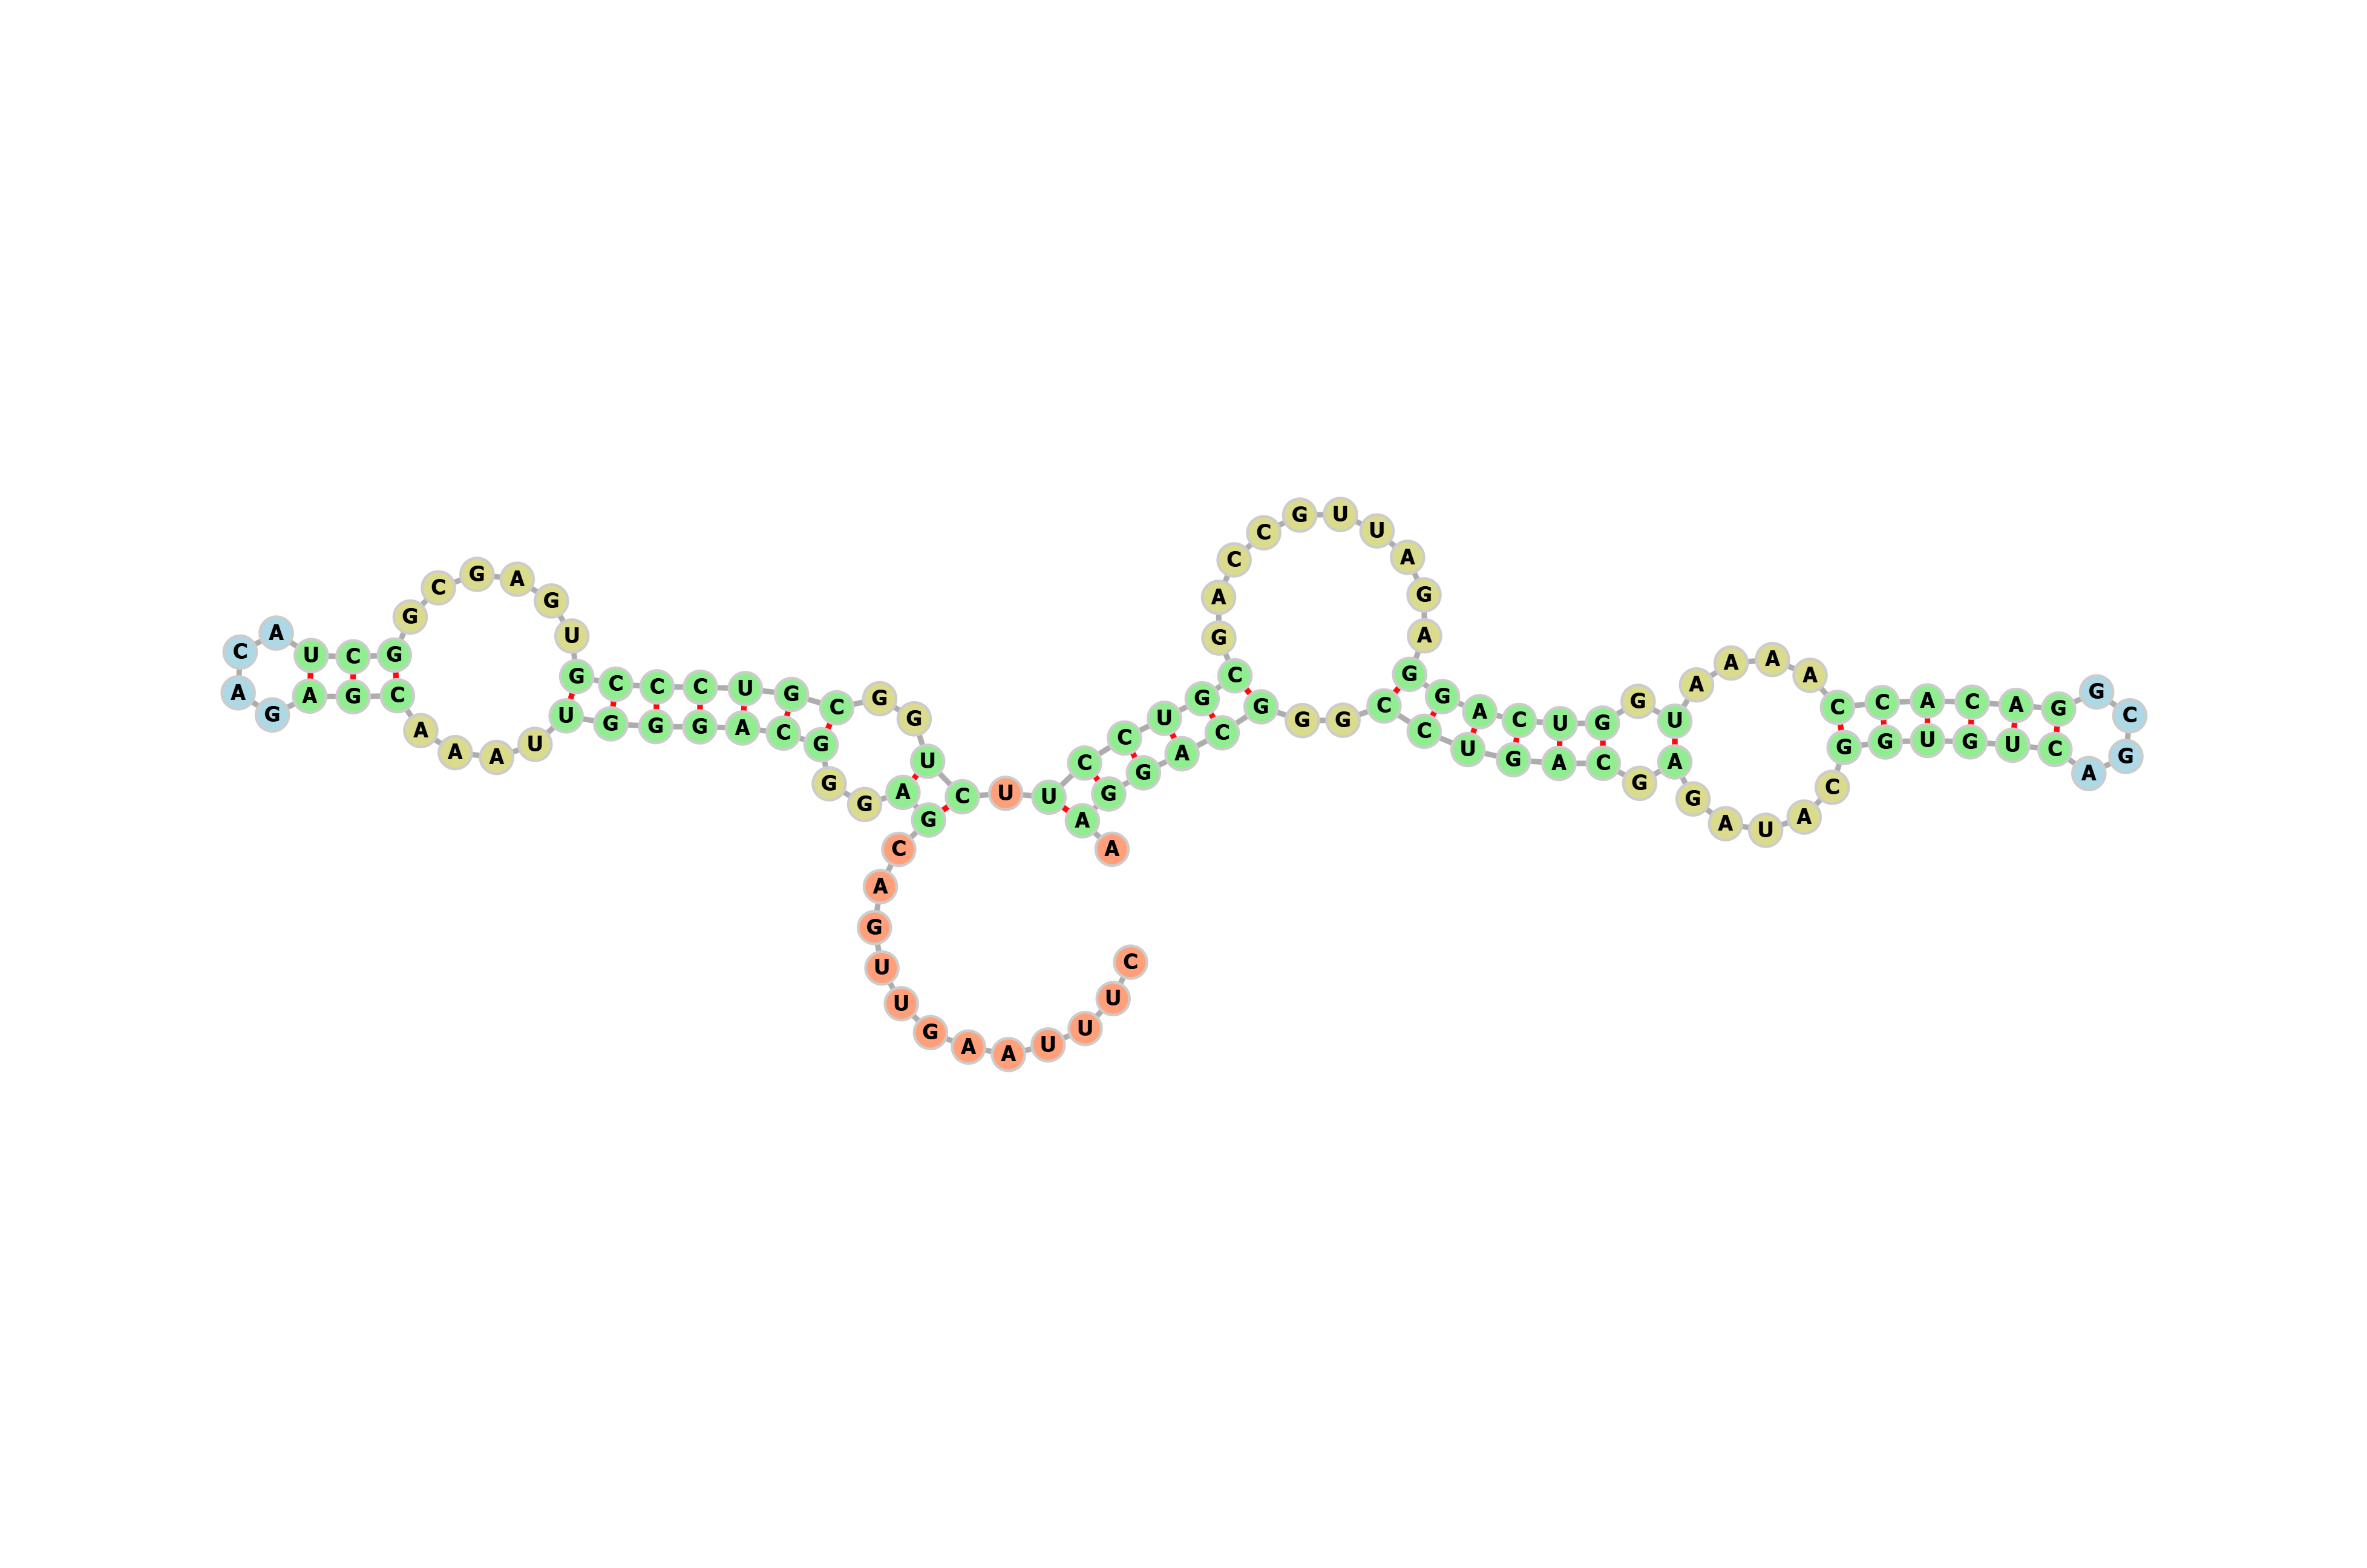
\includegraphics[width=\textwidth]{images/2d_case/native.png}
        \caption{Native (Ground Truth)}
    \end{subfigure}
    \hfill
    \begin{subfigure}[b]{0.32\textwidth}
        \centering
        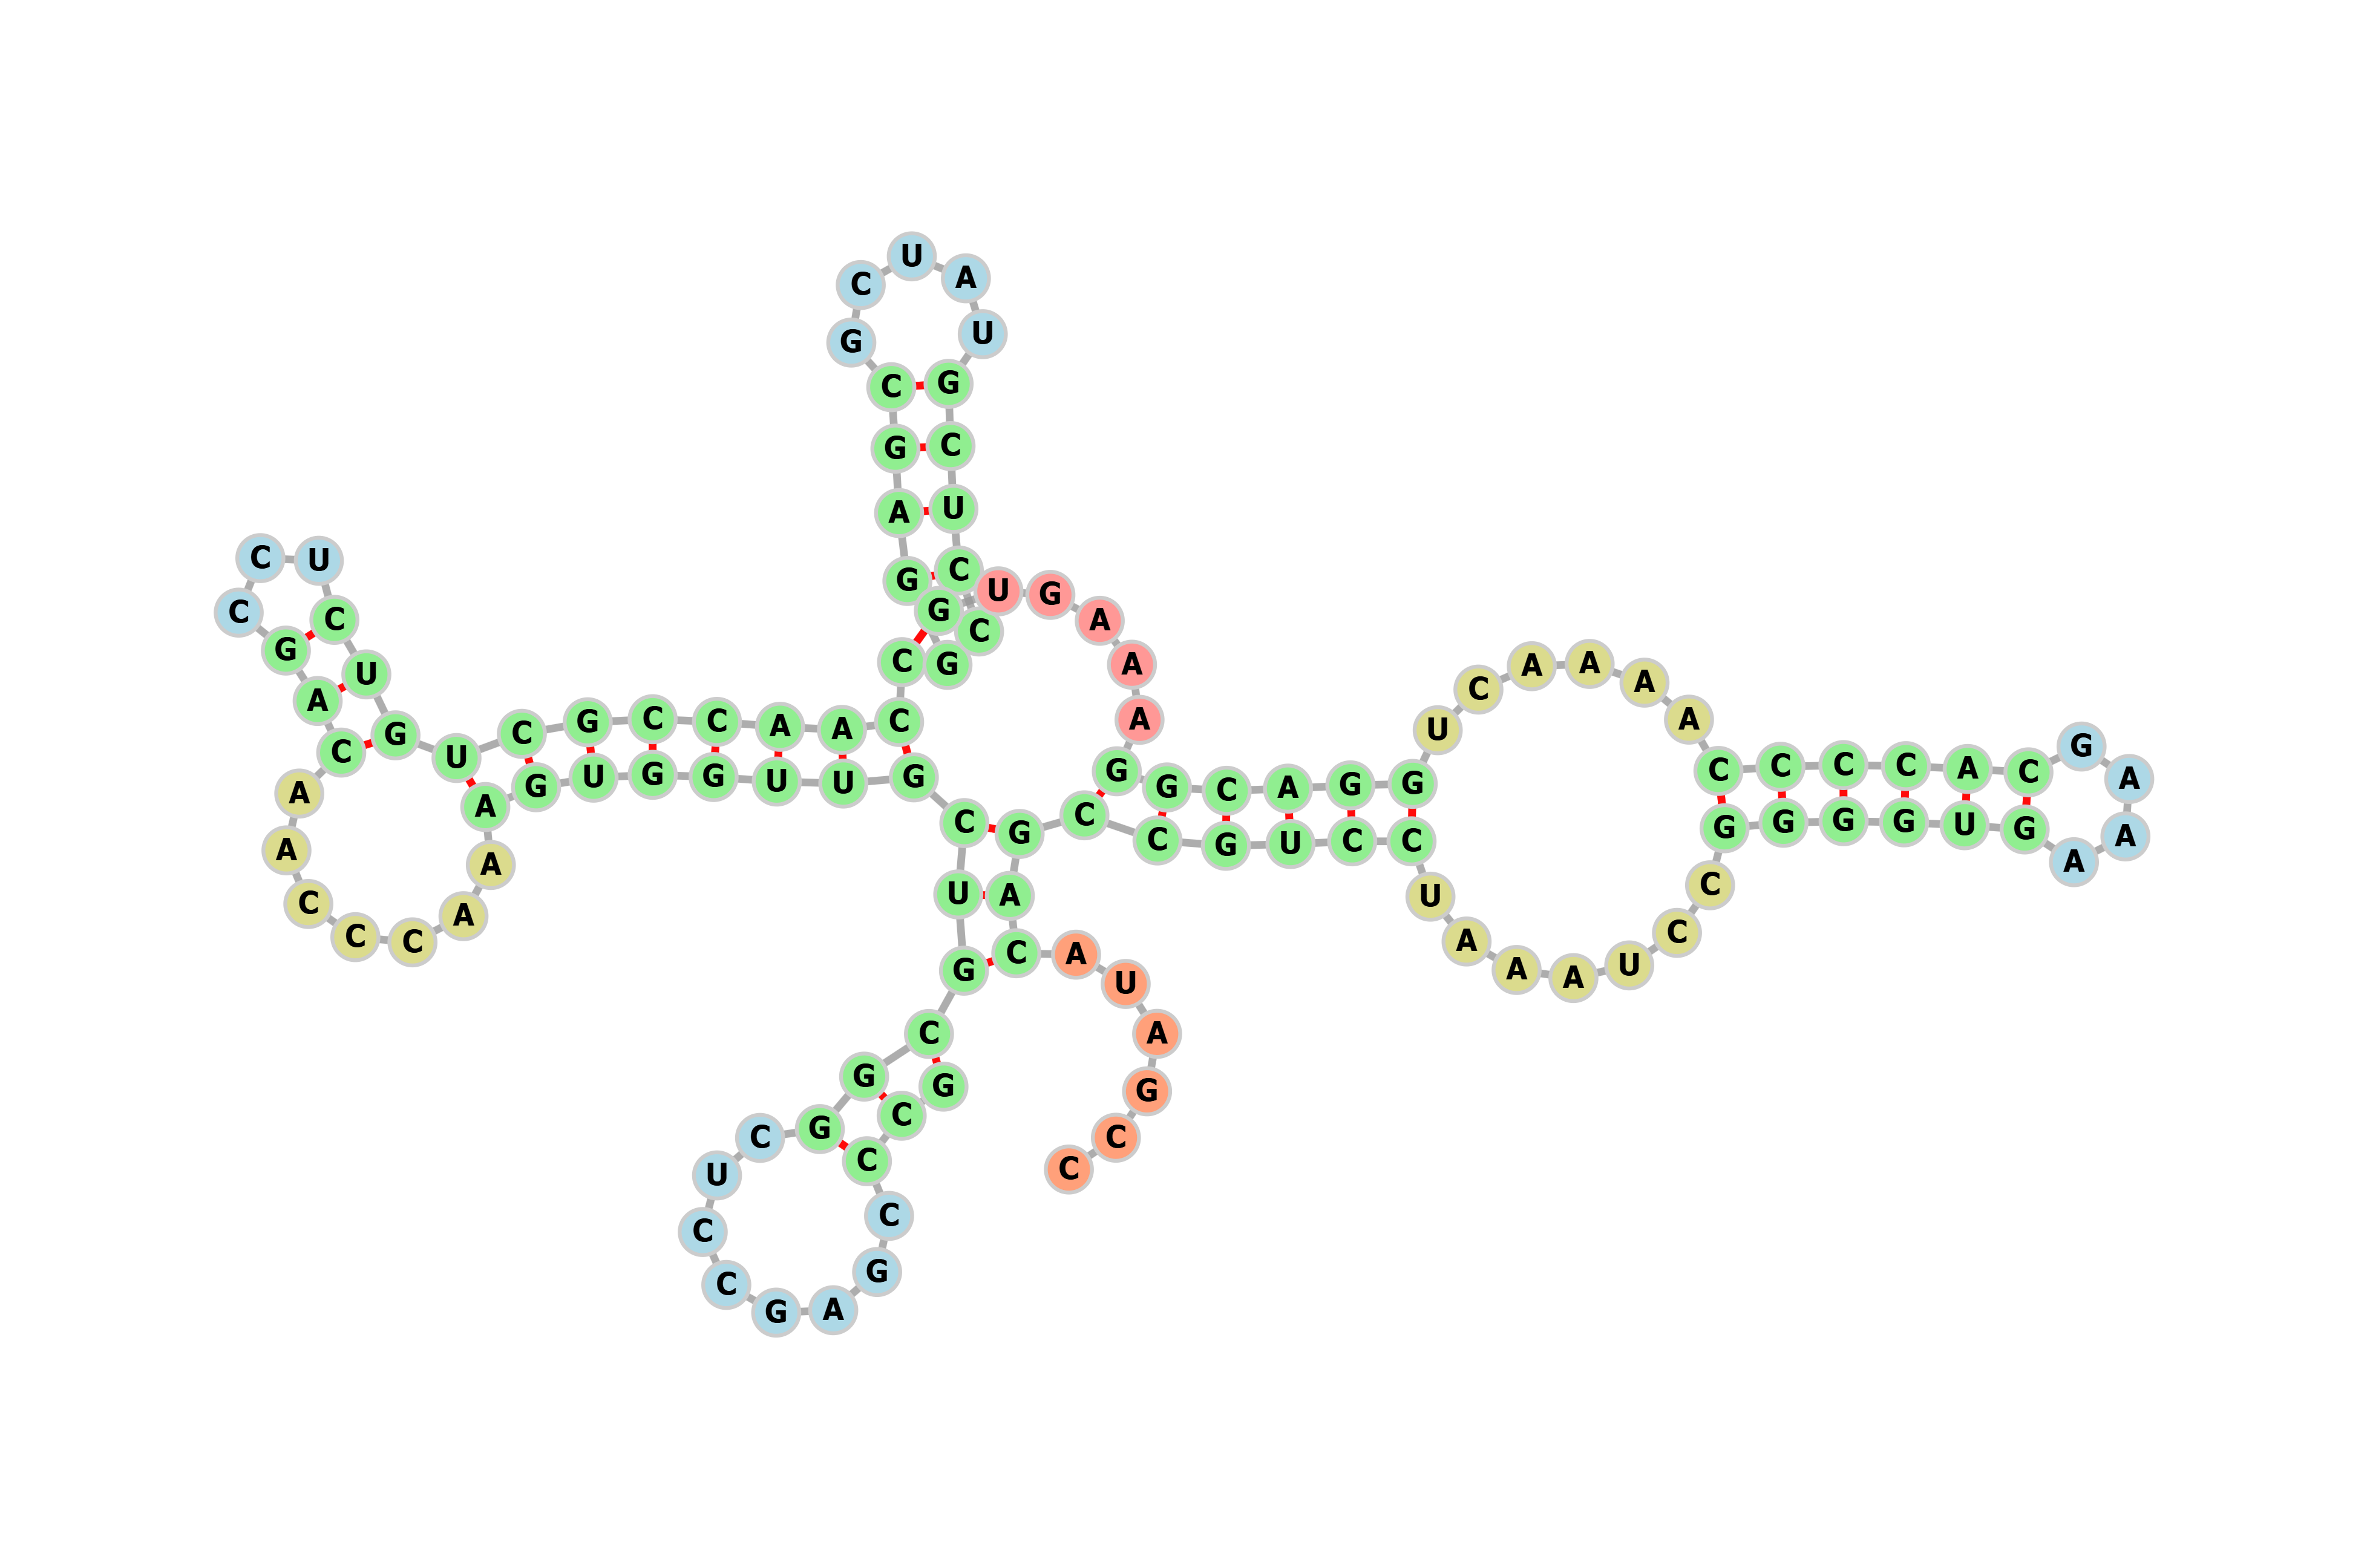
\includegraphics[width=\textwidth]{images/2d_case/grnade.png}
        \caption{gRNAde (Baseline)}
    \end{subfigure}
    \hfill
    \begin{subfigure}[b]{0.32\textwidth}
        \centering
        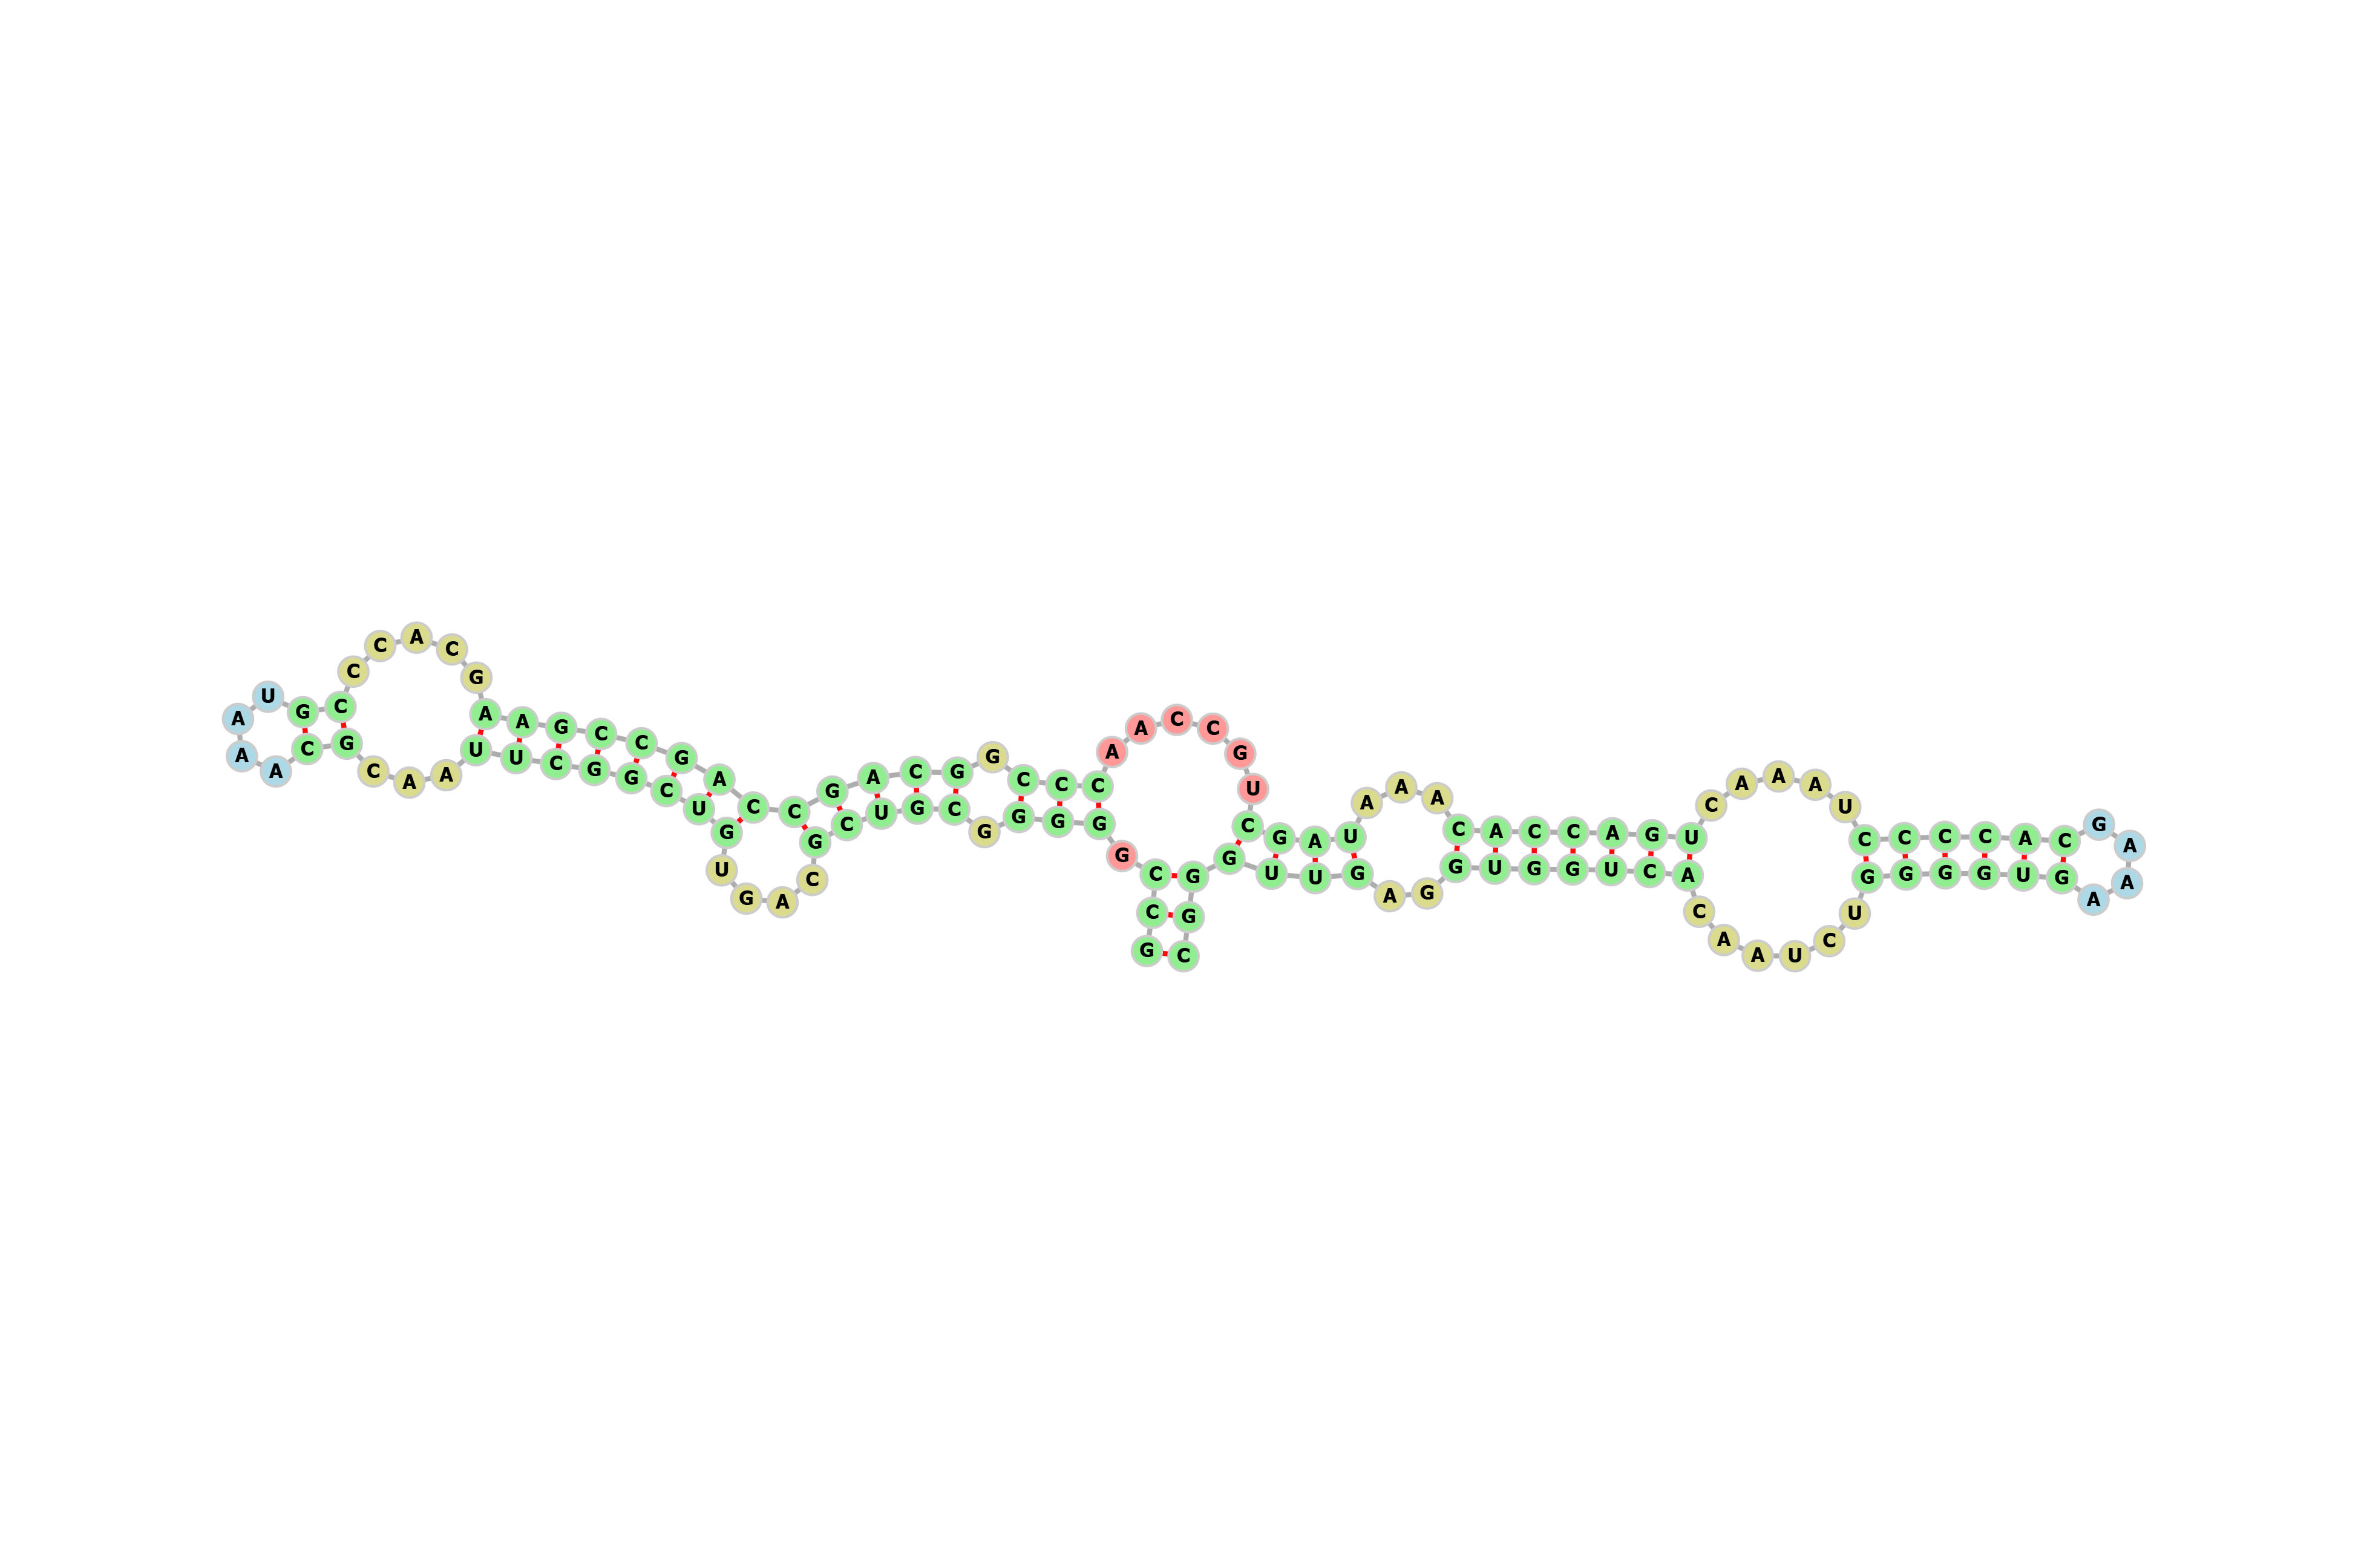
\includegraphics[width=\textwidth]{images/2d_case/ribopo.png}
        \caption{RiboPO (Ours)}
    \end{subfigure}
    \caption{Comparison of 2D Secondary Structures. While gRNAde hallucinates a complex multi-way junction, RiboPO correctly identifies the native linear topology, demonstrating superior designability.}
    \label{fig:2d_comparison}
\end{figure}

% --- Figure 2: 3D Structure Comparison ---
\begin{figure}[H]
    \centering
    \begin{subfigure}[b]{0.48\textwidth}
        \centering
        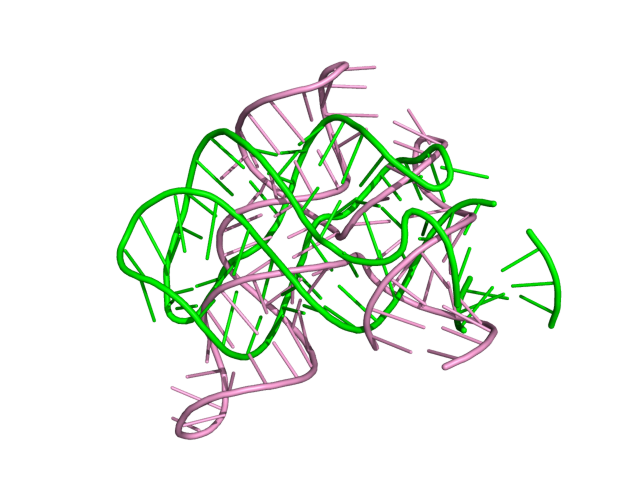
\includegraphics[width=\textwidth]{images/3d_case/superpose_grnade.png}
        \caption{gRNAde vs. Native (Seq Rec. = 0.446, TMscore = 0.060, RMSD = 18.455)}
    \end{subfigure}
    \hfill
    \begin{subfigure}[b]{0.48\textwidth}
        \centering
        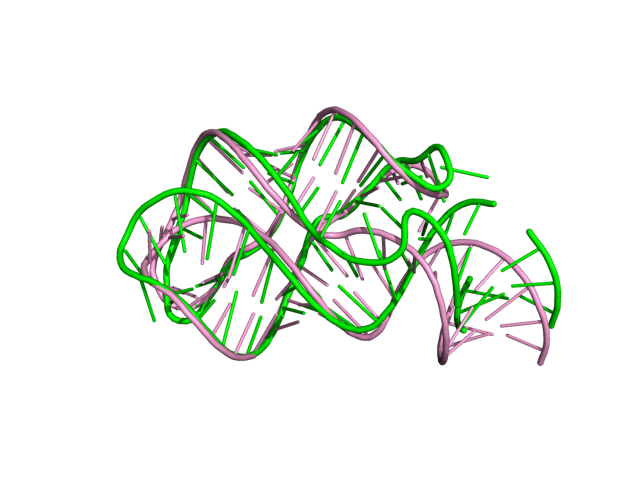
\includegraphics[width=\textwidth]{images/3d_case/superpose_ribopo.png}
        \caption{RiboPO vs. Native (Seq Rec. = 0.446, TMscore = 0.462, RMSD = 3.684)}
    \end{subfigure}
    \caption{3D Structure Superposition (Green: Native, Pink: Designed). RiboPO achieves significantly better alignment and domain orientation compared to the baseline, correcting the global fold errors.}
    \label{fig:3d_comparison}
\end{figure}
}

\subsection{LLM Usage}
We utilized a large language model to assist with improving the grammar, spelling, and overall clarity of the manuscript. The scientific contributions, including all ideas, methods, and results, are our own. We take full responsibility for the content of this paper.






